\documentclass[letterpaper,11pt]{article}

\usepackage{ucs}
\usepackage[utf8x]{inputenc}
\usepackage{graphicx}
\usepackage{amsfonts}
\usepackage{dsfont}
\usepackage{amssymb}
\usepackage{amsmath}
\usepackage{amsthm}
\usepackage[titletoc]{appendix}

\usepackage{enumerate}
\usepackage{stmaryrd}
\usepackage{fullpage}
\usepackage{ifthen}
\usepackage{subfigure}
\usepackage{epic}
\usepackage{authblk}
\usepackage{textcomp}
\usepackage[small]{caption}
\SetSymbolFont{stmry}{bold}{U}{stmry}{m}{n}

\usepackage{enumitem}

\usepackage[hypertexnames=false,colorlinks=true,linkcolor=blue,citecolor=blue]{hyperref}
\usepackage[numbers,comma,square,sort&compress]{natbib}
\usepackage[letterpaper,text={7in,9in},centering]{geometry}

\usepackage{bm}
\usepackage{color}
\usepackage{titlesec}
\setlength{\parindent}{0.0in}
\setlength{\parskip}{1.0ex plus0.2ex minus0.2ex}
\renewcommand{\baselinestretch}{1.1}
\graphicspath{{eps/}{pdf/}}
\setcaptionmargin{0.25in}
\def\captionfont{\itshape\small}
\def\captionlabelfont{\upshape\small}

\renewcommand{\labelenumi}{(\roman{enumi})}

\newcommand{\bqq}{\begin{equation}}
\newcommand{\eqq}{\end{equation}}
\newcommand{\bqs}{\begin{equation*}}
\newcommand{\eqs}{\end{equation*}}

\newcommand{\Ral}{\mathcal{R}}


\newcommand{\C}{\mathbb{C}}
\newcommand{\D}{\mathbb{D}}
\newcommand{\N}{\mathbb{N}}
\newcommand{\R}{\mathbb{R}} 
\newcommand{\Z}{\mathbb{Z}}

\newcommand{\rme}{\mathrm{e}}
\newcommand{\rmi}{\mathrm{i}}
\newcommand{\rmd}{\mathrm{d}}
\newcommand{\rmo}{{\scriptstyle\mathcal{O}}}
\newcommand{\rmO}{\mathcal{O}}
\newcommand{\eps}{\varepsilon}
\newcommand{\lar}{ \lesssim }


\newcommand{\Rho}{\bm{\rho}}
\newcommand{\bigma}{\bm{\sigma}}
\newcommand{\diag}{\operatorname{diag}}
\newcommand{\supp}{\operatorname{supp}}

\renewcommand{\qedsymbol}{$\blacksquare$}


\numberwithin{equation}{section}

\newenvironment{Hypothesis}[1]%
  {\begin{trivlist}\item[]{\bf Hypothesis #1 }\em}{\end{trivlist}}

\renewcommand{\arraystretch}{1.25}



% Define Theorem Styles ----------------------------------
\theoremstyle{plain}
\newtheorem{theorem}{Theorem}[section]
\newtheorem{proposition}[theorem]{Proposition}
\newtheorem{lemma}[theorem]{Lemma}
\newtheorem{corollary}[theorem]{Corollary}
\newtheorem{conjecture}[theorem]{Conjecture}
\newtheorem{main}[theorem]{Main Result}
\newtheorem{rmk}[theorem]{rmk}


\newcommand{\etal}{\textit{et al.}\ }

\newcommand{\greg}[1]{%
  {\color{blue}\textbf{Greg:} #1}%
 }
 
\newcommand{\arnd}[1]{%
  {\color{red}\textbf{Arnd:} #1}%
 }


\newenvironment{Proof}[1][.]%
 {\begin{trivlist}\item[]\textbf{Proof#1 }}%
 {\hspace*{\fill}$\rule{0.3\baselineskip}{0.35\baselineskip}$\end{trivlist}}

\renewcommand\labelitemi{$\bullet$}

\title{Passage through a fold without a phase space}
\author{author}
\date{2016}
\begin{document}
\begin{center}

{\fontsize{17}{17}\fontfamily{cmr}\fontseries{b}\selectfont{Alternatives to the blow-up method in singular perturbation problems}}\\[0.2in]
Arnd Scheel and Tianyu Tao\\
\textit{\footnotesize 
University of Minnesota, School of Mathematics,   206 Church St. S.E., Minneapolis, MN 55455, USA}
\date{\small \today} 
\vspace*{0.2in}
\end{center}

\begin{abstract}
\noindent We revisit the classical problem of determine the asymptotic expansion of the solution near the passage of a fold point in a singularly perturbed system, where the theory of normally hyperbolic invariant manifold cannot be directly applied, the standard remedy is the blow-up method first demonstrated by Krupa and Szmolyan. In this paper we show how one can use a functional analytic approach to achieve the same goal.
\end{abstract}

\section{Introduction}
In this paper we study singularly perturbed ordinary differential equations (ODEs) of the form

\begin{align}\label{intro_slow}
\begin{split}
\eps \dot{x} &=  f(x,y;\eps),\\
\dot{y } &=   g(x,y;\eps),   
\end{split}\hspace{0.2in} x\in \mathbb{R}^n, \hspace{0.2in} y \in \mathbb{R}^m, \hspace{0.2in} 0<\eps \ll 1,
\end{align}
where $f$ and $g$ are $C^k$ functions for $k>=3$.

The standard way of studying \eqref{intro_slow} is using methods from geometric singular perturbation theory. An brief overview of this theory involves treating system \eqref{intro_slow}, which is referred to as the \textit{slow-system}, together with its  equivalent counterpart, the \textit{fast-system}:
\begin{align}\label{intro_fast}
\begin{split}
x' &=  f(x,y;\eps),\\
y' &=  \eps g(x,y;\eps),   
\end{split}
\end{align}

where if $\tau$ denotes the (slow) time variable in system \eqref{intro_slow}, then $t = \tau/\eps$ is the (fast) time variable used in system \eqref{intro_fast}. The dynamics can then be studied by setting $\eps = 0$ in both systems to obtain the so-called \textit{reduced problem}
\begin{align}\label{intro_reduced}
\begin{split}
0 &=  f(x,y,0),\\
\dot{y} &=   g(x,y,0),   
\end{split}
\end{align}

and the \textit{layer problem}
\begin{align}\label{intro_layer}
\begin{split}
x' &=  f(x,y,0),\\
y' &=  0. 
\end{split}
\end{align}
The basic premise of the theory, which was first laid out by Fenichel, is that the dynamics of reduced problem \eqref{intro_reduced} happens on the \textit{critical manifold}
\[
S:=  \{ (x,y) \mid f(x,y;0) = 0 \},
\]
one then focuses on a \textit{normally hyperbolic submanifold} of equlibra $S_0 \subset S$ of the layer problem \eqref{intro_layer}, which will perturb to a so-called ``slow manifold'', $S_\eps$ for $0<\eps \ll 1$, on which the dynamics of \eqref{intro_slow} is an $\eps$-perturbation of the reduced problem \eqref{intro_reduced}. In addition to the existence of a slow manifold, we have the existence of stable and unstable invariant foliation along with base $S_0$, which also persists for $\eps>0$. More details can be found in \cite{Jones_GSPT} or \cite{chris_kuehn_book}, for example.

The above approach relies heavily on the notion of normal hyperbolicity, which may not be always satisfied in the problems to be studied. The most common case is the so-called \textit{fold point}, where the critical manifold $S$ loses its normal hyperbolicity near bifurcation points due to a zero eigenvalue in the Jacobian $\frac{\partial f }{\partial x}$.

To overcome these difficulties, Krupa and Szmolyan proposed the method of \textit{blow-up} to extend the reach of geometric singular perturbation theory in \cite{KrupaSz}. Roughly speaking, it is a set of coordinate transformations which desingularizes the vector field near the fold point so that information can be gained by using standard tools in dynamical system.


For fold points, their example was the following extended system 
\begin{align}\label{ori_eqn}
\begin{split}
u' &= \mu+u^2+ f(u,\mu; \eps),\\
\mu' &=  \eps g(u,\mu; \eps), \\
\eps' &= 0
\end{split}
\end{align}
where $(\mu, u, \eps)$ in a sufficiently small neighborhood $\mathcal{U}$ of the origin so that the critical manifold 
\[
S_0 = \{ (\mu, u) \mid \mu + u^2 +f (u,\mu ;0) = 0\}
\]
 has only $(0,0)$ as the fold point.
 Further, a generic condition on the nonlinearity $f, g$ are assumed, so that they have the following expansions
\begin{equation} \label{fold_nonlinearity}
f(u,\mu;\eps) = \rmO(\eps, u\mu,\mu^2,u^3),\hspace{0.2in}
g(u,\mu;\eps) = 1+\rmO(u,\mu,\eps),
\end{equation} 
for $(\mu, u,\eps) \in \mathcal{U}$.

\begin{figure}[ht]
 \centering % centering figure
 \scalebox{0.3} % rescale the figure by a factor of 0.3
 {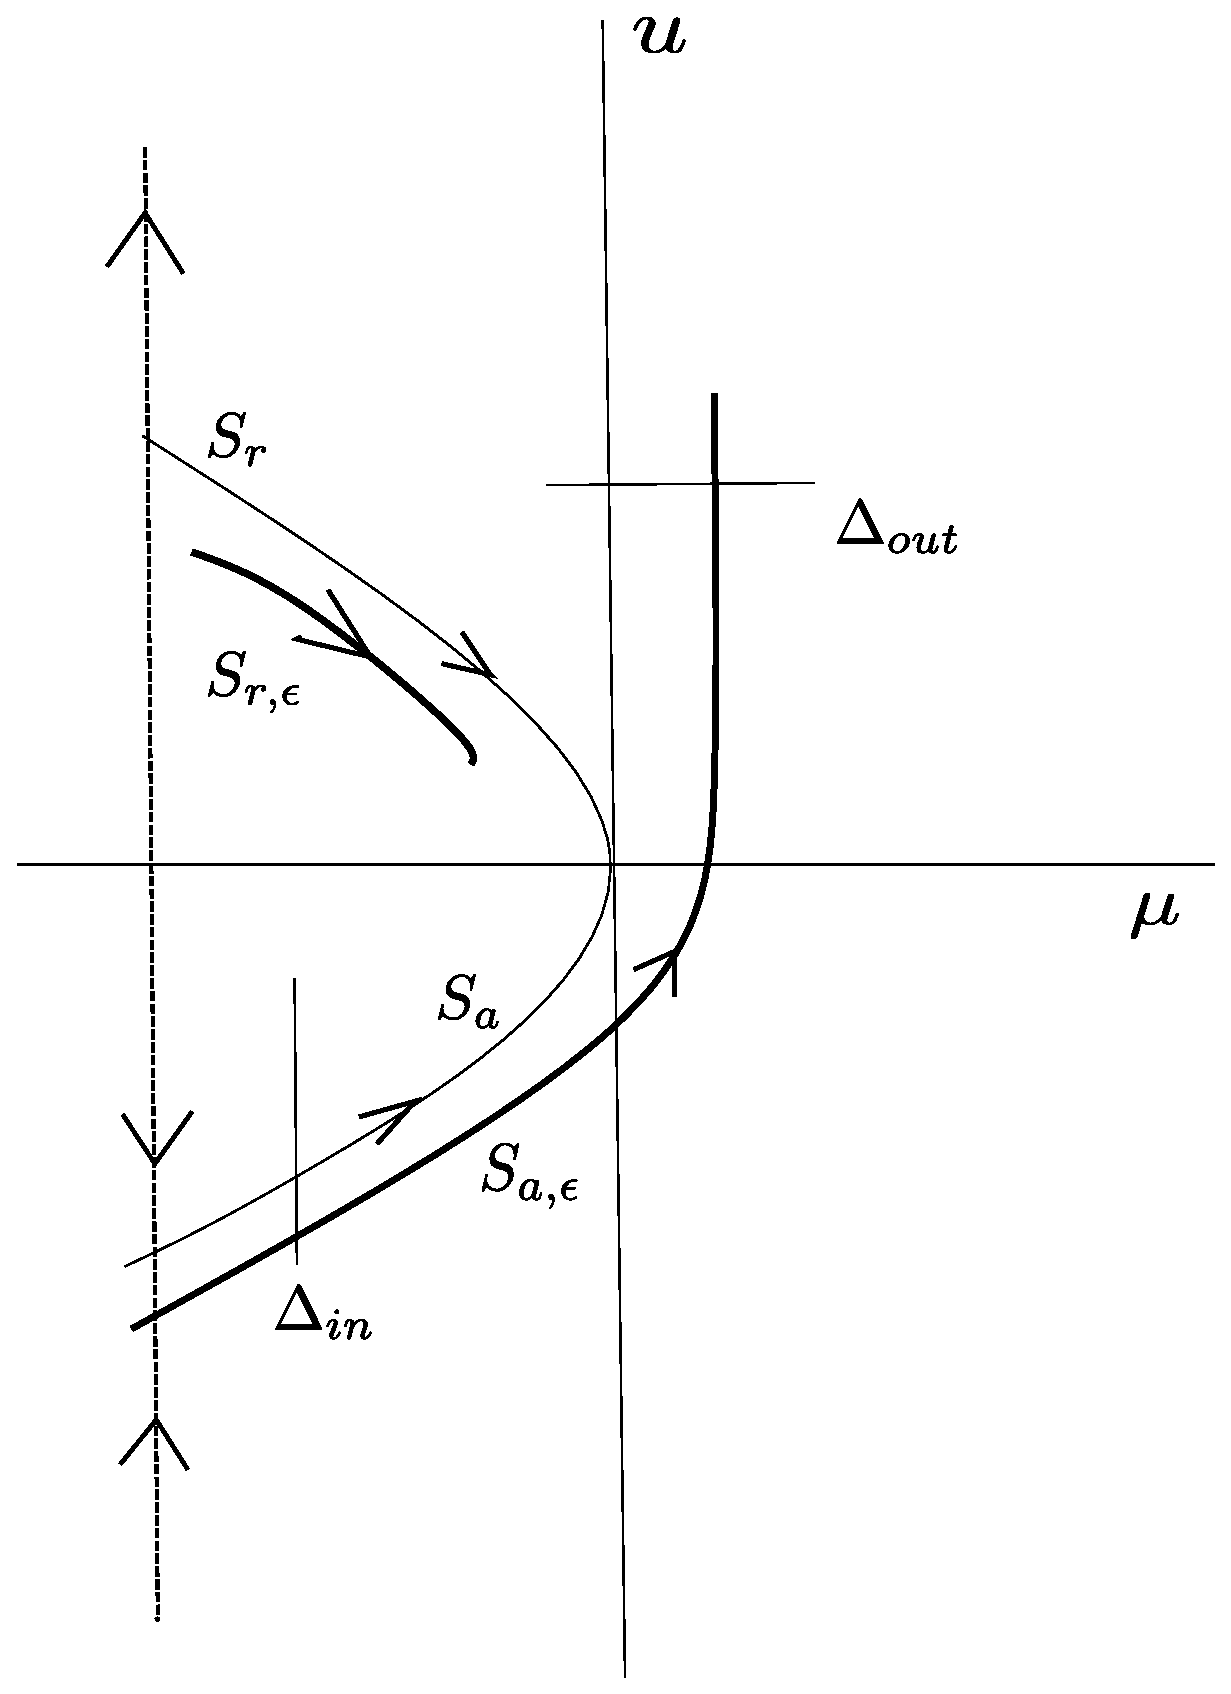
\includegraphics{pictures/passage_fold.eps}} % importing figure
 \caption{critical manifold and slow manifolds, section near the fold}\label{fig:passage}
\end{figure}

 Away from the fold point $(0,0,0)$, there exist the attracting manifold $M_a$ with a section $S_a$ sketched in Figure \ref{fig:passage}. By standard Fenichel's theory, $S_a$ perturbs to $S_{a,\eps}$ until it reaches the fold point, thus a natural question is to track how a trajectory starting on the slow manifold $S_{a,\eps}$ passes through the fold point.

Krupa and Szmolyan starts by setting two sections $\Delta_{in} = \{(-\delta, u) \mid u\in J,\text{ $J$ is some small interval }\}$ and $\Delta_{out} = \{( \mu ,\sqrt{\delta})\mid \mu \in \mathbb{R})\}$ with $\delta>0$ small but fixed, which are also shown in figure \ref{fig:passage}. To track the passage through the fold amounts to study the transition map 
\[
\pi: \Delta_{in} \to \Delta_{out},
\]

Krupa and Szmolyan then proceed by defining the blow up transformation
\[
u =\bar{r} \bar{u},  \quad \mu = \bar{r}^2 \bar{\mu}, \quad  \eps = \bar{r}^3 \bar{\eps},
\]
which ``blows up'' the vector field of the extended $(\mu, u, \eps)$ system near $(0,0,0)$ into a vector field on the ball $B = S^2 \times [0,\eps_0^{1/3}] \ni (\bar{u}, \bar{\mu}, \bar{\eps}, \bar{r})$ for some $\eps_0>0$ small, and further directional blow-ups to obtain charts $K_1,K_2,K_3$ which was used to describe the flows in regions near different parts of the manifold $B$. After a careful and thorough analysis, they were able to prove the following results:
\begin{theorem}\label{ks_main}(Theorem 2.1 in \cite{KrupaSz})

For $\eps$ sufficiently small, the following statements are true:
\begin{enumerate}
\item The manifold $S_{a,\eps} $ passes through  $\Delta_{out}$ at a point $(h(\eps), \sqrt{\delta})$ where $h(\eps) = \rmO(\eps^{2/3})$.
\item The transition map $\pi$ is a contraction with rate $\rmO(e^{-c/\eps} )$, where $c$ is a positive constant independent of $\eps$.
\end{enumerate}
\end{theorem}


In this paper, we focus on the same problem \eqref{ori_eqn} with an aim to recreate the result of Theorem \ref{ks_main} via a different, functional-analytical approach. Instead of proceeding with the geometrically-flavored blow-up approach, we directly prove a trajectory exists with the properties claimed in Theorem \ref{ks_main} by dividing the time of passage into appropriate parts and setting up a corresponding ansatz in each region, closing the arguments with carefully reformulating the existence question as a fixed-point argument.

\paragraph{Outline}
The reminder of the paper is organized as follows. In Section \ref{sec_main} we give a precise statement of our result, as well as an overview of our set ups. In Sections \ref{sec_A}, \ref{sec_B} and \ref{sec_C} we construct the ansatz mentioned earlier and in Section \ref{sec_glue} we show how to piece together all the parts to arrive at our main results.


\paragraph{Notation}We use the notation $\mathcal{C}^k(a,b)$ to denote the space of functions with $k$ continuous derivatives on the interval $(a,b)$ for $k\ge 0$.  
We use $A \lar B$ to indicate that there is a constant $C$ such that $A \le C \cdot B$, independent of the properties of $A$ and $B$. We also use the brackets $\langle x \rangle$ to represent the expression $\sqrt{x^2+1}$. We also use $\|A\|_{X\to Y}$ to denote the usual operator norm for the linear operator $A: X\to Y$ which maps from the function space $X$ into $Y$:
\[
\|A\|_{X\to Y} := \sup_{ x\neq 0} \frac{\|Ax\|_Y}{\|x\|_X}.
\]



\section{Main Result}\label{sec_main}
Wwe first make a change of variable to transform equation \eqref{ori_eqn} into a more convenient form in Section \ref{euler_m}. Then we introduces the different ansatz used in Section \ref{Ric_def} and \ref{c_mfld}. We then give a statement of our main result in Section \ref{main_sum} and in Section \ref{t_sigma} we explain how we divide up the passage time into 3 different regions $A$, $B$, and $C$ to prepare for the proof of this theorem.

\subsection{Euler multiplier}\label{euler_m}
Let $\tau$ denote the independent time variable in \eqref{ori_eqn}, since for $u,\mu,\eps$ small, $g(u,\mu,\eps) = 1 + \rmO(u,\mu,\eps)>0$, we can define a new time $t = t(\tau)$ by $\frac{dt}{d\tau} = g$, consequently, equation \eqref{ori_eqn}  is transformed into
\begin{align}\label{euler_ori_eqn}
\begin{split}
\frac{d}{dt}u &= \mu+u^2+ \tilde{f}(u,\mu;\eps),\\
\frac{d}{dt}\mu &=  \eps ,
\end{split}
\end{align}
where now $\tilde{f}$ satisfies the asymptotics
\begin{equation}\label{nonlinear_asy_new}
\tilde{f}(u,\mu,\eps) = \rmO(\eps,  u\mu, \mu^2,\eps u, \eps \mu, \eps u^2, u^3).
\end{equation}  

The critical manifold 
\[
\tilde{S}_0 = \{ (\mu, u) \mid \mu + u^2 + \tilde{f}(u,\mu;0) = 0\},
\]
still has $(0,0,0)$ as the only fold point, and our goal is to track how a trajectory of the flow of \eqref{euler_ori_eqn} passes through the fold. Following the set up of the sections $\Delta_{in}$ and $\Delta_{out}$ in Krupa-Szmolyan, we propose the following boundary conditions

\begin{equation}\label{ori_bc}
\mu(0) = -\delta_-, \hspace{0.2in} u(T) = \delta_+,
\end{equation}
where $T$ is also an unknown variable which marks the ``time of exit'' as the trajectory hits the section $\Delta_{out}$, and $\delta_{\pm}$ are small positive numbers.

That is, we think the tracking of the passage of the fold as a shooting problem, if we can prove the existence of a solution $(\mu, u)$ to system \eqref{euler_ori_eqn} with the boundary condition \eqref{ori_bc}, and give the expansion for the components $\mu$, then we will prove the results in \eqref{ori_eqn}. Our contribution in this paper is that the method we used to prove the existence of such a solution is different than the blow-up approach.

In the rest of the paper, we shall drop the tilde to use $f(u,\mu,\eps)$ as the nonlinearity and $S_0$ to denote the critical manifold.



\subsection{The Riccati equation}\label{Ric_def}
First, we want to get an idea of what kinds of ansatz one should use. Consider \eqref{euler_ori_eqn} with $f(u,\mu;\eps) = 0$, which can then be scaled such that $\eps = 1, \mu = s$, and 
\begin{equation}\label{ric}
\frac{d}{ds}u(s) = s+u(s)^2,
\end{equation}

which is the Ricatti equation in its simplest form. We denote any solution to \eqref{ric} as $u_R$, it is known to have a unique solution (denoted by $\bar{u}_R$) with the following asymptotic expansions (see \cite{KrupaSz} as well).

\begin{equation} \label{ric_asy}
\bar{u}_R(s)=\begin{cases}
  (\Omega_0-s)^{-1}+\rmO(\Omega_0-s), \text{ as }s \to \Omega_0, \\
 -(-s)^{1/2} -\frac{1}{4}(-s)^{-1} + \rmO(|s|^{-3/2}), \text{ as }s \to -\infty.
\end{cases}
\end{equation}

Here the constant $\Omega_0 \approx 2.3381$ is the smallest positive zero of 
\[
J_{-1/3}(2z^{3/2}/3)+J_{1/3}(2z^{3/2}/3),
\]
where $J_{\pm 1/3}$ are Bessel functions of the first kind.


More generally, we consider family of solutions  $u_R(s; u_0)$ of the Riccati equation  \eqref{ric} such that $u_R(0; u_0) = u_0$. That is, we take the initial condition $u_0$ as a parameter to the Riccati equation. For the special Riccati solution $\bar{u}_R$, we denote $\bar{u}_R(0) $ as $\bar{u}_0$. In fact, using simple phase plane analysis, we can extend the asymptotic results about the special Riccati solution $\bar{u}_R$, \eqref{ric_asy} to the $u_0$-parameter dependent family $u_R(s; u_0)$, as the following proposition states.

\begin{proposition}\label{para_ric}
There exist $\eta>0$ small, so that for all initial condition $u_0$ with $|u_0- \bar{u}_0|<\eta$, there exist a number $\Omega_\infty=\Omega_\infty(u_0)$ which depends on $u_0$ smoothly, and a solution $u_R(s;u_0)$ of \eqref{ric} on $[0, \Omega_\infty(u_0))$ with the following asymptotic expansion as $s\to \Omega_\infty(u_0)$:
\begin{equation}\label{ric_exp}
u_R(s;u_0) = \frac{1}{\Omega_\infty-s} +  (\Omega_\infty-s) r(\Omega_\infty-s;u_0),
\end{equation}
where the function $r$ is smooth in both variables and satisfies
\begin{equation}\label{ric_reminder}
r( \Omega_\infty-s; u_0) = -\frac{\Omega_\infty}{3} + \rmO(\Omega_\infty-s),
\end{equation}
as $s \to \Omega_\infty$.
\end{proposition}
we postpone the proof of this proposition to the appendix.
\subsection{Critical manifold}\label{c_mfld}
Another piece of the ansatz comes from part of  the critical manifold, we expect this because away from the fold, the critical manifold has an attracting branch $S_a$ which implies trajectory has to stay close to it. 

Recall the critical manifold for system \eqref{crit_mfld} is the set of points $(\mu, u) $ in a small neighborhood of the origin which satisfies
\begin{equation} \label{crit_mfld}
\mu + u^2 + f(u,\mu; 0) =  0.
\end{equation}

From \eqref{nonlinear_asy_new} we see that $\mu = -u^2+\rmO(u^3)$, by rescaling $\mu = -\mu_1^2$ with $\mu_1$ positive and $u=\mu_1 u_1$ we obtain
\[
u_1^2 = 1 + \rmO(\mu_1),
\]
and hence two branches of solutions
\[
u_1 = \pm \sqrt{1}+\rmO(\mu_1) \implies u = \pm \sqrt{-\mu}+\rmO(\mu).
\]

We therefore define
\begin{align}
\begin{split}
u_-(\mu) &= -\sqrt{-\mu} + \rmO(|\mu|),\\
u_+(\mu) &= +\sqrt{-\mu} + \rmO(|\mu|).
\end{split}
\end{align}


In particular, we set
\begin{equation}\label{singular}
u_s(t)=u_-(\mu(t)) ,
\end{equation}
so that
\[
0 = \mu(t) + u_s^2(t)+f(u_s(t),\mu; 0).
\]
Due to the simple form of \eqref{euler_ori_eqn} and \eqref{ori_bc}, we have that $\mu(t)= \eps t-\delta_-$, hence $u_s(\mu)$ satisfies
\begin{equation}\label{singularAsy}
u_s(t) = -\sqrt{\delta-\eps t} + \rmO(|\delta-\eps t|).
\end{equation}


\subsection{Main result - summary} \label{main_sum}

We now state our main result. Recall $\mathcal{U}$ is a neighborhood small enough so that \eqref{fold_nonlinearity} holds for $(\mu, u , \eps) \in \mathcal{U}$.

\begin{theorem}\label{thm:main}Let $\Omega_0$ be the constant defined in \eqref{ric_asy}.
Fix $\delta_-, \delta_+>0$ and $\alpha$ with $0<\alpha <3/4$. There exist $\eps_0>0,$ a constant $C=C(\delta,\alpha),$ such that for all $0<\eps<\eps_0$ and $u_i$ with $|u_i -u_-(-\delta) | \le C\eps^{1-\alpha/3}$, a solution of the rescaled system 
\begin{equation}\label{main_eqn}
\begin{split}
\frac{d}{dt}u &= \mu+u^2+ f(u,\mu;\eps), \\
\frac{d}{dt} \mu &= \eps.  \\
\end{split}
\end{equation}
with the initial condition
\begin{equation}\label{main_ic}
\begin{split}
u(0) &= u_i, \\
\mu(0) &= -\delta_-,
\end{split}
\end{equation}

exists for $t \in (0,T)$, where the end point $T$ is the desired ``exit time'' in the sense that 
\begin{equation}\label{exit_time_cond}
 u(T) = \delta_+.
\end{equation}

Moreover, $T$ has the following expansion in $\eps$:
\begin{equation}\label{T_exp_+}
T = T(\eps ; u_i) = \eps^{-1}\delta_- + \eps^{-1/3}\Omega_0 +  \mathcal{H}(\eps; u_i),
\end{equation}
with the term $\mathcal{H}(\eps;u_i)$ satisfies 
\begin{equation}\label{T_remainder_exp}
\eps\mathcal{H}(\eps;u_i) = \rmO(\eps^{1-\alpha/3}), \hspace{0.2in} \text{Lip}_{u_i}\eps\mathcal{H}(\eps;u_i) = \rmO(1).
\end{equation}
In particular, since $\mu(t) = \eps t -\delta_-$, we have the following expansion of the exit location $\mu(T)$ on the section $\Delta_{out}$ in $\eps$:
\begin{equation}\label{exit_loc_exp}
\mu(T) = \eps^{2/3}\Omega_0  + \eps\mathcal{H}(\eps; u_i) = \eps^{2/3}\Omega_0 + \rmO(\eps^{1-\alpha/3})
\end{equation}

\end{theorem}

To fully recover Theorem \ref{ks_main}, we have the following corollary.
\begin{corollary}\label{cor:main}
For $\alpha,\delta_-,\delta_+>0$, there is a compact interval $K \subset (-\infty, u_+(-\delta_-))$, independent of $\eps$ so that for all $u_i \in K$ with $(u_i,\mu,\eps) \in \mathcal{U}$, the same conclusion of Theorem \ref{thm:main} holds. In fact, there exist a constant $c$ independent of $\eps$, such that the Lipschitz constant of $\mathcal{H}(\eps;u_i)$ in the expansion \eqref{T_exp_+} satisfies
\begin{equation}\label{T_remainder_exp_+}
\text{Lip}_{u_i} \eps\mathcal{H}(\eps;u_i) = \rmO(e^{-c/\eps}),
\end{equation}
for all $u_i \in K$.
\end{corollary}



\textbf{Remark:} Notice $\alpha>0$ could be chosen arbitrary small in the expansion \eqref{exit_loc_exp}. In fact, it is well-known from the matched-asymptotics community that the next order term after $\eps^{2/3}\Omega_0$ is of order $\eps \log(\eps)$.  This is also confirmed in \citep{KrupaSz} using the blow-up methods. 


 The proof of Theorem \ref{thm:main} and \ref{cor:main} will take up the rest of the paper,  we first prepare ourselves with the setup of the problem in the following sections.

\subsection{Division of regions and the rescaling of time}\label{t_sigma}
Now that we can introduce the ansatz. We divide the time from $t=0$ to $t=T$ into three ``Regions'' where we take a different ansatz on each region. 

We first start with the exit time $t=T$ when the trajectory hits the section $\Delta_{out}$. Also, we use $T$ to mark the rightmost boundary of the region $A$, where our proposed solution takes the form
\[
u_A(t; u_0) = u_*(t;u_0)  + w_r(t;u_0),
\]
here the function $u_* = u_*(t; u_0)$ is defined as:
\begin{equation}\label{urdef}
u_*(t; u_0) := \eps^{1/3}u_R(\eps^{1/3}(t-\eps^{-1}\delta_-); u_0),
\end{equation}
where $u_R=u_R(s; u_0)$ is the family of solutions to the Riccati equation which were shown to exist in Proposition \ref{para_ric}, it solves the initial value problem
\begin{equation}\label{ureq}
\frac{d}{dt}u_*(t; u_0) = \mu(t) + u_*^2(t; u_0), \hspace{0.2in} u_*(\eps^{-1}\delta_-; u_0) = \eps^{\frac{1}{3}} u_0,
\end{equation}
with $\eps$ and $u_0$ as parameters.  The function $w_r$ is a correction term whose properties will be given in later sections. 

In region $A$, the ansatz $u_*(t)$ is merely a rescaled version of the Riccati solution $u_R(s; u_0)$, which follows the first half of the asymptotic expansion in Proposition \ref{para_ric}. When $u_*(t)$ start to be controlled by the other part of the asymptotic expansion, we will need to adaptively change our ansatz or function space in order to ``glue'' the solutions, an intuitive, but rather arbitrary place to switch regions is at $t = \eps^{-1} \delta_-$. This marks the start of region $B$, where our choice of solution is as follows:
 \[ 
 u_B(t) = \bar{u}_*(t)  +w_\ell(t).
\]
Where $\bar{u}_*$ is the function
\begin{equation}\label{uldef}
\bar{u}_*(t) = u_*(t;\bar{u}_0) = \eps^{1/3} u_R( \eps^{1/3}(t-\eps^{-1}\delta_-); \bar{u}_0)=\eps^{1/3}\bar{u}_R(\eps^{1/3}(t-\eps^{-1}\delta_-)),
\end{equation}
and $\bar{u}_*$ solves the equation
\begin{equation}\label{uleq}
\frac{d}{dt}\bar{u}_* (t) = \mu(t) + \bar{u}_*^2(t),
\end{equation}
so similarly $\bar{u}_*$ is a rescaled version of the special solution to the Riccati equation. Also similar to the situation in region $A$, $w_\ell$ is a correction term whose properties will be described later.

The next piece of the ansatz will be used to connect the piece $u_B$, which roughly follows the special Riccati solution $\bar{u}_R$, to the attracting branch $S_a$ of the critical manifold $S_0$, a natural ``gluing point'' is where the error between $\bar{u}_*(t)$ and $u_s(t)$ defined in \eqref{singular} and \eqref{uldef}, is small. Calculation shows that this is at a point $t=t^*$ where we roughly have
\begin{equation}
(\delta_- - \eps t^*) \approx -\eps^{1/2},
\end{equation} 

hence we choose $t^*$ as a natural transition point from region $B$ to the last region, region $C$, where it covers the rest of the passage time until at $t=0$. The corresponding solution will take the form
\[
u_C(t) = u_s(t) + w_s(t),
\]
the $w_s(t)$ is yet another correction term whose properties will be discussed later. 

In summary, region $A$, $B$ and $C$ are divided as follows:
\begin{align}\label{region_division_t}
\begin{split}
\text{Region A:} & \quad (\eps^{-1}\delta_-, T), \quad \text{solution in region A:} \quad u_A(t) = u_*(t)+w_r(t), \\
\text{Region B:} & \quad (t^*, \eps^{-1}\delta_-), \quad \text{solution in region B:} \quad u_B(t) = \bar{u}_*(t)+w_\ell(t),  \\
\text{Region C:} & \quad (0, t^*), \quad \text{solution in region C:} \quad u_C(t) = u_*(t)+w_s(t).
\end{split}
\end{align}

Now we can briefly describe the strategy of our proof, we plug in the ansatz into equation \eqref{euler_ori_eqn} to derive the equation for the corrections $w_r, w_\ell $ and $w_s$, choose appropriate function space with norms and set up the equations for the corrections as fixed point argument on these function spaces. A main technical part of our proof consists of appropriately rescaling the time $t \in (0,T)$ so that we gain hyperbolicity in the sense that the linearized operator at the ansatz become Fredholm in the new time scale. This is the key observation in our approach, comparable to the blow-up approach which also gains hyperbolicity via a carefully chosen change of variable. Having solved for the correction terms $w_r, w_\ell$ and $w_s$, we can then collect information about their asymptotic expansion to confirm the corresponding solution has the properties we need.


Next, we describe how we transform time $t$ into time $\sigma$ to gain hyperbolicity. This is demonstrated in the following steps.
\begin{enumerate}
\item Step 1: Define $\psi$ as
\[
\psi = \eps^{1/3}(t - \eps^{-1}\delta_-),
\]

\item Step 2:
Fix $M>0$ large, define $\sigma$ as
\begin{equation} \label{psi_def}
\psi = \psi(\sigma; u_0) =\begin{cases}
-(-\frac{3}{2} \sigma)^{2/3} , &\text{ for }\sigma \le -M, \\
\Omega_\infty(u_0) -e^{-\sigma}, &\text{ for }\sigma \ge M,
\end{cases}
\end{equation}

here $\Omega_\infty$ is the blow-up time for $u_R$ found in Proposition \ref{para_ric}.

Also, we denote $\varphi(\sigma) := \frac{d}{d\sigma}\psi(\sigma)$, which has the following asymptotic expansions: 
\begin{equation} \label{phi_def}
\varphi(\sigma)  =\begin{cases}
(-\frac{3}{2} \sigma)^{-1/3} , &\text{ for }\sigma \le -M, \\
e^{-\sigma}, &\text{ for }\sigma \ge M,
\end{cases}
\end{equation}
\item Step 3: For $\sigma \in (-M, M)$, we define $\psi(\sigma)$ as the straight line connecting the two points $(M, \Omega_\infty-e^{-M})$ and $(-M, -(\frac{3}{2}M)^{2/3})$. As a result, if we define $\sigma_m=\sigma_m(u_0)$ as the value of $\sigma$ such that $\psi(\sigma_m; u_0) = 0$, then we have 
\[
\frac{|\sigma_m - M|}{M} = \left| \frac{(\frac{3M}{2})^{2/3}-(\Omega_\infty-e^{-M})}{(\frac{3M}{2})^{2/3}-(\Omega_\infty+e^{-M})} -1 \right|\le CM^{-2/3},
\] 
for some constant $C$ independent of $u_0$.

Therefore we can write
\begin{equation}\label{sigm_asy}
\sigma_m = M + M_r, \hspace{0.2in} |M_r| \le CM^{1/3}.
\end{equation}
\end{enumerate}

After defining the time transformation, the original exit time $t=T$ will be transformed into $\sigma=\sigma_T$ under this change of variable, and similarly the boundary between region $A$ and region $B$ is  transformed from $t=\eps^{-1}\delta_-$ to $\sigma = \sigma_m$ and the boundary between region $B$ and region $C$ is  transformed from $t=t^*$ to $\sigma = \sigma^*$, and $t=0$ into $\sigma = \sigma_0$. We will see later that the $\sigma_0, \sigma^*, \sigma_m, \sigma_T$ satisfies:
\[
\sigma _0 \approx -\delta_-^{3/2}\eps^{-1}, \quad \sigma ^* \approx -\eps^{-1/4}, \quad \sigma_m = \rmO_\eps(1), \quad
\sigma_T \approx -\log(\eps^{1/3}\delta_+^{-1}) 
\]
In summary, the regions in time $\sigma$ are as follows:
\begin{align}\label{region_division_sig}
\begin{split}
\text{Region A:} & \quad (\sigma_m ,\sigma_T ),  \\
\text{Region B:} & \quad (\sigma^*, \sigma_m),  \\
\text{Region C:} & \quad (\sigma_0, \sigma^*),
\end{split}
\end{align}
and the following picture summarizes the relationship between the two time scales $t$ and $\sigma$, as well as the corresponding regions divided. 

\begin{figure}[ht]
 \centering % centering figure
 \scalebox{0.6} % rescale the figure by a factor of 0.3
 {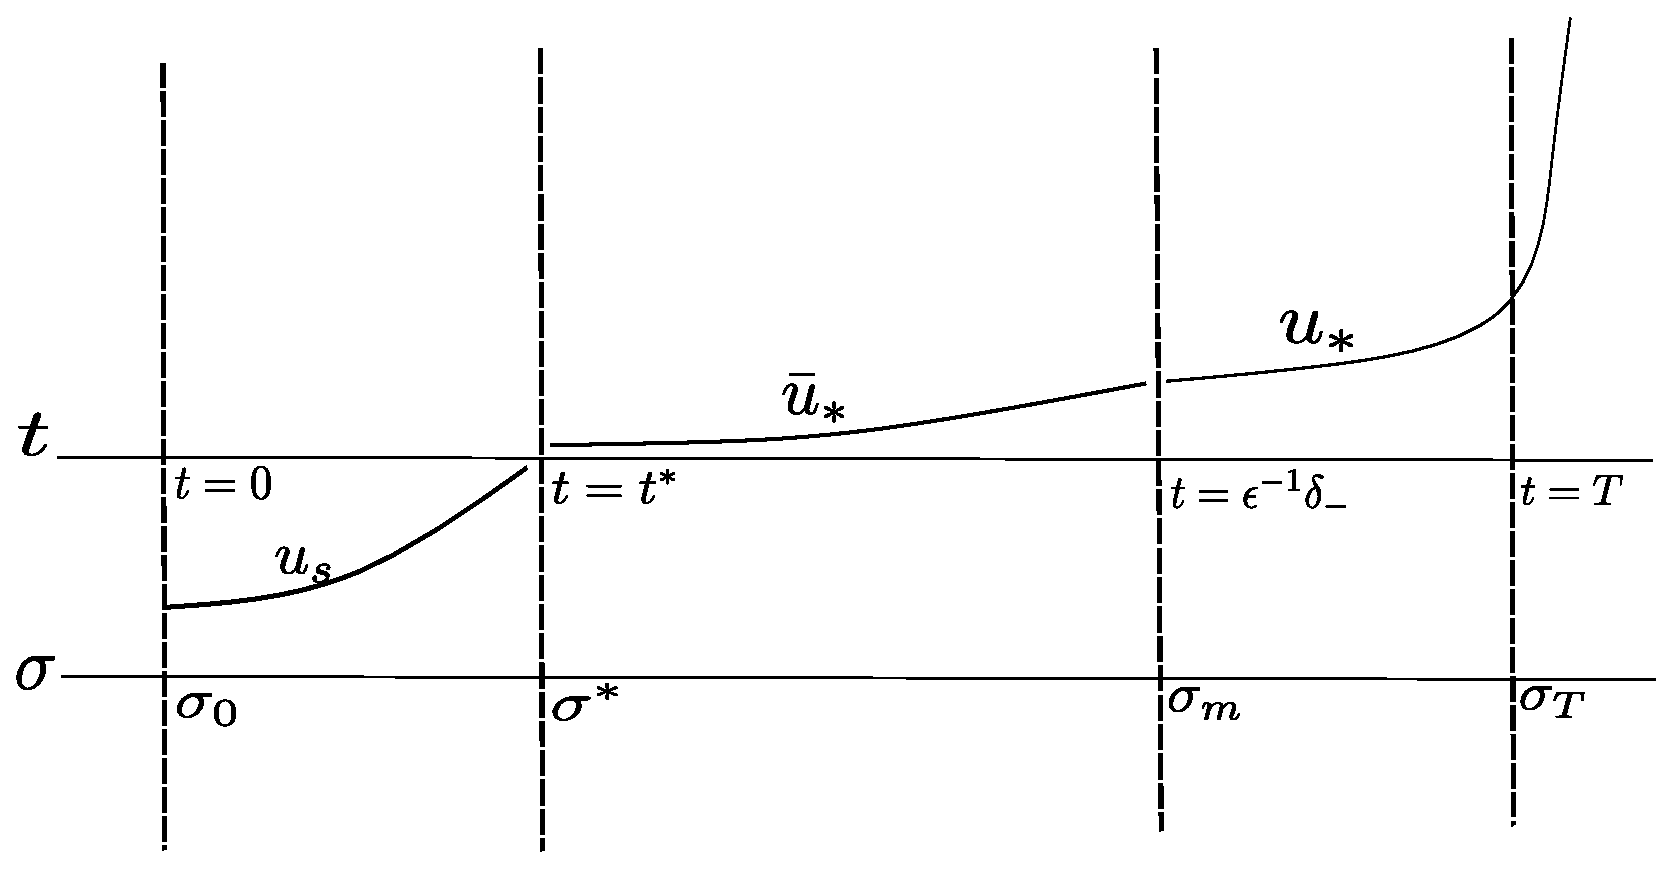
\includegraphics[angle = 0, origin = c]{pictures/time_scale.eps}} % importing figure
 % labeling to refer it inside the text
 \caption{Time scales used to divide the regions.}
\end{figure}\label{fig:time_scale} 


\section{Region A}\label{sec_A}

Region A corresponds to the time-$t$ interval $\{ t : t > \eps^{-1}\delta_-\}$. In this section we will give the precise form of the solution which solves system \eqref{euler_m} on this region.

\subsection{Solution in region A}

\begin{theorem}\label{thm:r}
Fix $\alpha>0, \delta_-,\delta_+>0, \eta>0$ small enough, there exists $\eps_A>0$ and a constant $C=C(\alpha,\delta_-,\delta_+,\eta)$, such that for all $0<\eps <\eps_A$, and all $|u_0 - \bar{u}_0|<\eta$, there exist a time $T=T(\eps;u_0)$, such that a solution of the form
\begin{equation}
u_A(t;u_0) = u_*(t; u_0) + w_r(t; u_0),
\end{equation}
to the rescaled system \eqref{main_eqn} exists on the time interval $t \in (\eps^{-1}\delta_-, T)$,
where
\begin{equation}
u_*(t; u_0) = \eps^{1/3}u_R(\eps^{1/3}(t-\eps^{-1}\delta_-); u_0),
\end{equation} and $u_R(\cdot; u_0)$ is the family of solution to Riccati equation that were shown to exist in Proposition \ref{para_ric}. 

Moreover, we have
\begin{enumerate}[label=\textnormal{(\arabic*)}]
\item \label{thm:r_1}$T=T(\eps;u_0) = \eps^{-1}\delta_-+\eps^{-1/3}\Omega_\infty(u_0)-\delta_+^{-1}+T_r$ with $T_r = \rmO( \eps^{2/3}\delta_+^{-3} )$ where the constant $\Omega_\infty(u_0)$ is defined in Proposition \ref{para_ric};
\item \label{thm:r_2} $w_r(T; u_0) = 0$ and $u_*(T,u_0)=\delta_+$;

\item \label{thm:r_3} if we define  
\begin{equation}\label{def:T_inf}
T_\infty = T_\infty(\eps; u_0) := \eps^{-1}\delta_- + \eps^{-1/3}\Omega_\infty(u_0),
\end{equation}
then $w_r$ is continuous with $|w_r(t; u_0)| \le C|T_\infty-t|^{\alpha-2}$ for $t \in (\eps^{-1}\delta_-, T)$;

\item \label{thm:r_4} the function 
$\Psi: (\bar{u}_0-\eta, \bar{u}_0+\eta) \to \mathbb{R}$ defined by $\Psi(u_0)=  w_r(\eps^{-1}\delta_-; u_0)$ is Lipschitz continuous, with Lipschitz constant 
\[
|\text{Lip}_{u_0}\Psi |\le C\eps^{(2-\alpha)/3}. 
\]
\end{enumerate}
\end{theorem}

We will prove this theorem in the following sections.
\subsection{The exit time \texorpdfstring{$T(u_0)$}{T(u_0)}}\label{exit_time}
Take $\eta>0$ so that the function $u_R = u_R(\cdot; u_0)$ exists for $|u_0-\bar{u}_0|<\eta$ as demonstrated in Proposition \ref{para_ric}. The exit time $T$ is then defined by the condition 
\[
\delta_+ = u_*(T; u_0) = \eps^{1/3}u_R(\eps^{1/3}(T-\eps^{-1}\delta_-); u_0).
\]
Recall the expansion for $u_R$ as formula given in \eqref{ric_exp}. If we define $\psi_T = \eps^{1/3}(T-\eps^{-1}\delta_-)$, then $\psi_T$ satisfies
\[
\frac{1}{\Omega_\infty-\psi_T} + (\Omega_\infty-\psi_T)r(\Omega_\infty-\psi_T) = \eps^{-1/3}\delta_+,
\]
from which we obtain the leading order expansion $\Omega_\infty-\psi_T = \rmO(\eps^{1/3}\delta_+^{-1})$. A fixed point argument gives
\[
\Omega_\infty - \psi_T = \eps^{1/3}\delta_+^{-1} + \rmO(\eps \delta_+^{-3}).
\]
Hence, the expansion for $T=T(\eps; u_0)$ becomes
\begin{equation}\label{T_exp}
T = T(\eps;u_0) = \eps^{-1}\delta_- + \eps^{-1/3}\Omega_\infty(u_0) - \delta_+^{-1} + T_r(\eps;u_0),
\end{equation}
with 
$|T_r|\le C\eps^{2/3}\delta_+^{-3}$, for some constant $C$ independent of $u_0$, as $\eps \to 0$.


\subsection{Equation for \texorpdfstring{$w_r$}{wr} and rescaling}\label{equation_wr}
We now substitute $u = u_* + w_r$ into equation \eqref{euler_m}, and obtain the equation for $w_r$
\begin{align}\label{eqn_wr}
\begin{split}
w_r' - 2u_*w_r &= w_r^2 + f(u_*+w_r, \mu; \eps) =: R_r(w_r; \eps,u_0).
\end{split}
\end{align}
Moreover, we enforce the boundary condition $u(T; u_0) = \delta_+$, which gives the boundary condition for $w_r$ at $t=T$:
\begin{equation}\label{Bc_w_r}
w_r(T;u_0) = 0.
\end{equation}

Therefore, we need to solve equation \eqref{eqn_wr} on the interval $t \in (\eps^{-1}\delta_-, T)$, with boundary condition \eqref{Bc_w_r}.

Next, we rescale equation \eqref{eqn_wr} into $\sigma$-time by using the $t$ to $\sigma$-time rescaling in Section \ref{t_sigma}, and obtain
\begin{equation}\label{rescl_wr}
\left(\frac{d}{d\sigma} - a(\sigma; u_0)\right) W_r =\eps^{-1/3}\varphi \mathcal{R}_r(W_r; \eps,u_0),
\end{equation}
where we have the following properties.
\begin{itemize}
\item The term $a(\sigma; u_0)$ satisfies
\begin{equation}\label{asy:a}
a(\sigma; u_0) := 2\varphi(\sigma)u_R(\psi(\sigma; u_0); u_0) =  2+\rmO(e^{-2\sigma}) \text{ as }\sigma \to \infty,
\end{equation}
where $\psi, \varphi$ were defined in equations \eqref{psi_def} and \eqref{phi_def} respectively. We remark that this convergence as $\sigma \to \infty$ is uniform in $u_0$ due to the definition of our time-rescaling.

\item The function $W_r(\sigma)$ is the rescaled version of $w_r(t)$ in the $\sigma$-variable, 
\[
W_r(\sigma): = w_r(\eps^{-1/3}\psi(\sigma)+\eps^{-1}\delta_-) = w_r(t) .
\] 

Similarly, $U_*$ is the rescaled version of $u_*$, with 
\[
U_*(\sigma;\eps,u_0) :=u_*(\eps^{-1/3}\psi(\sigma)+\eps^{-1}\delta_-;\eps,u_0)= \eps^{1/3}u_R(\psi(\sigma;u_0);u_0) = u_*(t;\eps,u_0).
\]

\item The function $\Ral_r$ is a rescaled version of $R_r$ such that 
\[
\mathcal{R}_r(W_r;\eps,u_0) := W_r^2 + f(U_*+W_r, \mu ; \eps),
\]
\end{itemize}
 
In order to obtain the boundary condition corresponding to equation \eqref{Bc_w_r}, we need to know the corresponding $\sigma$-time for the $t$-time interval $t\in (\eps^{-1}\delta_-, T)$.

At $t = \eps^{-1}\delta_-$, the corresponding $\sigma$ time is at $\sigma=\sigma_m$, from its definition in Section \ref{t_sigma}, with
\[
\sigma_m = M + \rmO(M^{1/3}) = \rmO(1),
\]
independent of $\eps$.

At $t=T$, we have $\eps^{1/3}(T-\eps^{-1}\delta_-) = \Omega_\infty -\eps^{1/3}\delta_+^{-1}+\eps^{1/3}T_r=\psi(\sigma_T) = \Omega_\infty-e^{-\sigma_T}$ from \eqref{T_exp}, hence, for $\eps$ small enough, we find that the $\sigma$-time corresponding to $t=T$ is 
\begin{equation}\label{def_sigm_T}
\sigma_T=\sigma_T(u_0;\eps) = -\log(\eps^{1/3}(\delta_+^{-1}-T_r)) = -\log(\eps^{1/3}\delta_+^{-1}) - \log(1-\delta_+ T_r(u_0;\eps)),
\end{equation}
where $T_r(u_0;\eps)$ is defined in equation \eqref{T_exp}.

In conclusion, the problem we want to solve is
\begin{align}\label{wr_bp}
\begin{split}
\frac{d}{d\sigma} W_r - a(\sigma;u_0)W_r &= \eps^{-1/3}\varphi \Ral_r(W_r), \text{ for } \sigma \in (\sigma_m, \sigma_T),\\
W_r(\sigma_T) &= 0.
\end{split}
\end{align}


\subsection{Linear equation and norms}


Our goal now is to solve \eqref{wr_bp} on an appropriate function space. to do so, we first slightly enlarge the time interval $(\sigma_m, \sigma_T)$ where the boundary value problem is posed.

From the definition of $\sigma_T$ \eqref{def_sigm_T}, we see that
\begin{equation}\label{sigm_T_asy}
|\sigma_T -(-\log(\eps^{1/3}\delta_+^{-1}))| \le |\log(1-\delta_+ T_r)| \le  C|\delta_+ T_r|\le C\eps^{2/3}\delta_+^{-2},
\end{equation} 
for some constant $C$ independent of $u_0$ provided that $|u_0-\bar{u}_0|<\eta$.

We now define $\sigma_{\inf}$ and $\sigma_{\sup}$ as follows:
\[
\sigma_{\inf} = \inf_{|u_0-\bar{u}_0|<\eta}\sigma_m(u_0), \hspace{0.3in} \sigma_{\sup} = \sup_{|u_0-\bar{u}_0|<\eta}\sigma_T(u_0).
\]
From the definition of $\sigma_m$ in Section \ref{t_sigma} and equation \eqref{sigm_T_asy} we have
\[
\sigma_{\inf} = M + \rmO(M^{1/3}), \hspace{0.2in} \sigma_{\sup} = -\log(\eps^{1/3}\delta_+^{-1}) + \rmO(\eps^{2/3}\delta_+^{-2}),
\]
fix $\alpha>0$, we introduce the following weighted function space:
\begin{align*}
\mathcal{C}_r=\mathcal{C}_r(\sigma_{\inf}, \sigma_{\sup}) &= \left\{ w(\sigma) \in \mathcal{C}(\sigma_{\inf}, \sigma_{\sup}) : \sup_{\sigma_{\inf} \le \sigma \le \sigma_{\sup} } \left|\eps^{(\alpha-2)/3} e^{(\alpha-2)\sigma}w(\sigma)\right| < \infty \right\}. \\
%--------------------------------------
\end{align*}


Next we study the linear operator $A_r=A_r(u_0,\eps)$ with
\[
A_r w = \left( \frac{d}{d\sigma}w-a(\sigma; u_0) w,  w(\sigma_T)\right),
\]
which is defined on a dense subset $\mathcal{D}(A_r) \subset \mathcal{C}_r$.

\begin{proposition}\label{inv_A_r}
The linear operator $A_r(u_0,\eps) : \mathcal{D}\subset \mathcal{C}_r \to \mathcal{C}_r\times \mathbb{R}$ is invertible, with its inverse 
\[
A_r^{-1}(u_0,\eps) : \mathcal{C}_r \times \mathbb{R} \to \mathbb{R}
\]
bounded uniformly in $u_0 \in (\bar{u}_0-\eta, \bar{u}_0+\eta)$ and $\eps \in (-\eps_A,\eps_A)$ with $\eta, \eps_A >0$ defined in Theorem \ref{thm:r}.

Moreover, we have the following estimate on the Lipschitz constant for the map $u_0 \mapsto A_r^{-1}(u_0,\eps)$.
\begin{equation}\label{Lip:Ar_inv}
\|A_r^{-1}(\tilde{u}_0,\eps) - A_r^{-1}(u_0,\eps)\|_{\mathcal{C}_r\times\mathbb{R}\to \mathcal{C}_r} \le C|\tilde{u}_0-u_0|
\end{equation}
for some constant $C$ independent of $\eps$.
\end{proposition}
\begin{Proof}
Consider the conjugate operator of $A_r$, given by
\begin{align*}
\tilde{A}_r v &= \left( e^{(\alpha-2)\sigma}\left(\frac{d}{d\sigma}-a(\sigma;u_0)\right)e^{(2-\alpha)\sigma} v, v(\sigma_T) \right) \\
&= \left( \frac{d}{d\sigma}v -(\alpha+a(\sigma;u_0)-2)v, v(\sigma_T) \right),
\end{align*}
which acts on $v(\sigma) \in \mathcal{C}^1(\sigma_{\inf}, \sigma_{\sup}) \subset \mathcal{C}(\sigma_{\inf}, \sigma_{\sup})$, with $v(\sigma) = \eps^{(\alpha-2)/3}e^{(\alpha-2)\sigma}w(\sigma)$. 

Consider the system 
\begin{align*}
\begin{split}
\frac{d}{d\sigma} w - a(\sigma;u_0)w &= f, \text{ for } \sigma \in (\sigma_m, \sigma_T),\\
w(\sigma_T) &= w_T.
\end{split}
\end{align*}
Which can be written as 
\[
A_r w = (f,w_T) \text{ with } f \in \mathcal{C}_r, w_T \in \mathbb{R}.
\] 

The conjugate system for $v$, which is 
\begin{align*}
\begin{split}
\frac{d}{d\sigma}v -(\alpha+a(\sigma;u_0)-2)v &= \tilde{f}, \text{ for } \sigma \in (\sigma_m, \sigma_T),\\
w(\sigma_T) &= v_T.
\end{split}
\end{align*}
Or equivalently written as
\[
\tilde{A}_r v = (\tilde{f},v_T),
\]
with $\tilde{f}(\sigma) = \eps^{(\alpha-2)/3}e^{(\alpha-2)\sigma} f(\sigma) \in \mathcal{C}(\sigma_{\inf}, \sigma_{\sup}),$ and $v_T = \eps^{(\alpha-2)/3} e^{(\alpha-2)\sigma_T}w_T$.
 
Then, from equation \eqref{asy:a} we see that the first component of $\tilde{A}_r$ converges uniformly as $\sigma \to \infty$ to the asymptotic operator 
\[
v\mapsto \left(\frac{d}{d\sigma} -\alpha \right) v.
\] 
Since $\alpha>0$, we may apply Lemma \ref{lin_bv} from the Appendix with $L= \sigma_T$ to conclude that there exists a constant $C$ independent of $\eps, u_0$ with 
\begin{equation}\label{linear_est:r}
\|w\|_{\mathcal{C}_r} = |v|_\infty \le C(|\eps^{(\alpha-2)/3}e^{(\alpha-2)\sigma} f |_{\infty}+|v_T|) \le C(\|f\|_{\mathcal{C}_r}+|w_T|).
\end{equation}
Notice that $|v_T| \le w_T$ by the asymptotic expansion of $\sigma_T  = \rmO(-\log(\eps^{1/3}))$. By the definition of $\sigma_{\inf}$ and $\sigma_{\sup}$, $A_r$ is uniformly invertible in the parameters $u_0,\eps$.

To show the Lipschitz estimates, we observe that if we take $f \in \mathcal{C}_r$ and $u_0, \tilde{u}_0 \in (\bar{u}_0-\eta, \bar{u}_0+\eta)$, then we have
\[
(A_r^{-1} -\tilde{A}_r^{-1})f = \tilde{A}_r^{-1}(\tilde{A}_r-A_r)A_r^{-1}f,
\]
where we abbreviated $A_r^{-1} = A_r^{-1}(u_0,\eps)$ and $\tilde{A}_r^{-1} = A_r^{-1}(\tilde{u}_0,\eps)$ and similarly for $A_r$. Since we just shown that $A_r^{-1}$ is uniformly bounded in $u_0$ and $\eps$, it suffices to estimate the Lipschitz constant for the map
\[
u_0 \mapsto A_r(u_0,\eps).
\]
However, by the definition of $A_r$, we have
\[
\|A_r-\tilde{A}_r\|_{\mathcal{C}_r\to \mathcal{C}_r\times \mathbb{R}} \le  \sup_{\sigma \in [\sigma_{\inf},\sigma_{\sup}]} |a(\sigma;u_0) - a(\sigma;\tilde{u}_0)|.
\]
where $a(\sigma; u_0) =  2\varphi(\sigma)u_R(\psi(\sigma;u_0);u_0)$ was defined in equation \eqref{asy:a}. Now we use the asymptotic expansion \eqref{ric_reminder} of $u_R$
\[
u_R(s;u_0) = \frac{1}{\Omega_\infty-s} +  (\Omega_\infty-s) r(\Omega_\infty-s;u_0),
\]
with the remainder function $r$ smooth in both of its arguments, to observe that
\[
\sup_{\sigma \in [\sigma_{\inf},\sigma_{\sup}]} |a(\sigma;u_0) - a(\sigma;\tilde{u}_0)|\lar 
\sup_{\sigma \in [\sigma_{\inf},\sigma_{\sup}]} |r(e^{-\sigma};u_0)-r(e^{-\sigma};\tilde{u}_0)|\le C|u_0-\tilde{u}_0|
\] 
for some constant $C$ independent of $\eps$. This shows the estimate \eqref{Lip:Ar_inv} and concludes the proof.
\end{Proof}

\subsection{Nonlinear estimates}

In this section we estimate the nonlinear term
\[
\mathcal{R}_r(W_r;\eps,u_0)(\sigma) = W_r^2(\sigma) + f(U_*(\sigma;\eps,u_0)+W_r(\sigma), \mu ; \eps),
\]
in the $\mathcal{C}_r$ norm to prove the following.
\begin{proposition}\label{nl_est_r}
If $W_r \in \mathcal{C}_{r}$, then $\eps^{-1/3}\varphi \mathcal{R}_r(W_r) \in \mathcal{C}_{r}$, and
\begin{equation}\label{nl_est:Rr}
\|\eps^{-1/3}\varphi \mathcal{R}_r(W_r) \|_{\mathcal{C}_r} = \rmO(\delta^{\alpha}).
\end{equation}
where $\alpha>0$ is a parameter in the definition of the function space $\mathcal{C}_r$.
Moreover, we have the following Lipschitz constant estimate for the map $W_r \mapsto \eps^{-1/3}\varphi\mathcal{R}_r(W_r)$.
\begin{equation}\label{Lip_est:Rr}
\|\eps^{-1/3}\varphi(\mathcal{R}_r(\widetilde{W}_r) - \mathcal{R}_r(W_r)) \|_{\mathcal{C}_r}\le C\delta^{1-\alpha} \|\widetilde{W}_r - W_r \|_{\mathcal{C}_r},
\end{equation}
for some constant $C$ independent of $\eps, \delta$.
\end{proposition}

\begin{Proof} Proposition \ref{ric_exp} shows that
\begin{equation} \label{u*_asy}
U_*(\sigma;u_0) =  \eps^{\frac{1}{3}}(e^\sigma+e^{-\sigma} r(e^{-\sigma}; u_0)   ) \text{ as }\sigma \to \infty,
\end{equation}
with the remainder function $r(\cdot;u_0)$ smooth in both arguments.
Therefore we have
\[
|U_*(\sigma)| \lar \eps^{\frac{1}{3}}e^\sigma \le \eps^{1/3}e^{\sigma_{\sup}} = \rmO(\delta_+),
\]
for all $\sigma \in [\sigma_{\inf},\sigma_{\sup}]$.

From the definition of the time rescaling in Section \ref{t_sigma} we have
\[
\mu = \eps t-\delta_-  =\eps^{2/3}\psi(\sigma) \lar \eps^{2/3},
\]
for all $\sigma \in [\sigma_{\inf},\sigma_{\sup}]$, since $|\psi(\sigma)| \le \Omega_\infty(u_0)$.

Since $W_r \in \mathcal{C}_r$, we have 
\[
|W_r(\sigma)| \lar \eps^{\frac{2-\alpha}{3}} e^{(2-\alpha)\sigma} \ll \eps^{1/3}e^\sigma, \text{ for } \sigma \in [\sigma_{\inf}, \sigma_{\sup}].
\]
which implies $|W_r(\sigma)| \lar |U_*(\sigma)|$ for $\sigma \in [\sigma_{\inf}, \bar{\sigma}_{\sup}]$, using the asymptotic expansion \eqref{u*_asy}.

Now we use the expansion \eqref{nonlinear_asy_new}
\[
f(u,\mu; \eps) = \rmO(\eps(1+u+\mu+u^2),u\mu,\mu^2,u^3)
\] 
and the fact that $U_*,W_r,\mu$ are all small in sup norm, to observe that
\begin{equation}\label{nonlinear_asy:fr}
f(U_*+W_r, \mu ;\eps) = \rmO(\eps, (U_*+W_r)\mu, \mu^2, (U_*+W_r)^3 ) = \rmO(\eps, U_*\mu, \mu^2, U_*^3).
\end{equation}

Using these facts, we have
\begin{equation}\label{nl_est:Rr_1}
\|\eps^{-\frac{1}{3}}\varphi W_r^2\|_{\mathcal{C}_r}=\sup |\eps^{-\frac{1}{3}} \varphi W_r| \lar \eps^{\frac{1-\alpha}{3}} e^{(1-\alpha)\sigma} \lar \eps^{\frac{1-\alpha}{3}} e^{(1-\alpha)\sigma_{\sup}} =  \rmO(\delta^{1-\alpha}_+),
\end{equation}

and
\[
\|\eps^{-1/3}\varphi f(U_*+W_r, \mu ;\eps)\|_{\mathcal{C}_r} \le \|\eps^{\frac{2}{3}}\varphi  \|_{\mathcal{C}_r}+\|\eps^{-\frac{1}{3}}\varphi U_*\mu \|_{\mathcal{C}_r}+\|\eps^{-\frac{1}{3}}\varphi \mu^2 \|_{\mathcal{C}_r}+\|\eps^{-\frac{1}{3}}\varphi U_*^3\|_{\mathcal{C}_r}.
\]

However we have
\[
\|\eps^{\frac{2}{3}}\varphi \|_{\mathcal{C}_r}=\sup |\eps^{\frac{2}{3}} \varphi   \eps^{(\alpha-2)/3}e^{(\alpha-2)\sigma}| \lar \eps^{\alpha/3} e^{(\alpha-3)\sigma_m} = \rmO(\eps^{\alpha/3}) ,
\]

\[
\|\eps^{-\frac{1}{3}}\varphi U_*\mu \|_{\mathcal{C}_r} =\sup |\eps^{-\frac{1}{3}} \varphi  U_*\mu  \eps^{(\alpha-2)/3}e^{(\alpha-2)\sigma} | \lar \eps^{\alpha/3} e^{(\alpha-2)\sigma_m}  =\rmO( \eps^{\alpha/3}) ,
\]

\[
\|\eps^{-\frac{1}{3}}\varphi \mu^2 \|_{\mathcal{C}_r} \lar \|\eps^{-\frac{1}{3}}\varphi \eps \|_{\mathcal{C}_r} \text{ since } \mu^2 = \rmO(\eps^{4/3}), 
\]
and
\[
\|\eps^{-\frac{1}{3}}\varphi U_*^3\|_{\mathcal{C}_r} \lar \eps^{\frac{\alpha}{3}} e^{\alpha\sigma} \lar \eps^{\frac{\alpha}{3}} e^{\alpha\sigma_{\sup}} = \rmO(\delta_+^\alpha).
\]

Therefore we conclude that
\begin{equation}\label{nl_est:Rr_2}
\|\eps^{-1/3}\varphi f(U_*+W_r, \mu ;\eps)\|_{\mathcal{C}_r} = \rmO(\delta^{\alpha}_+)
\end{equation}

Combining estimates \eqref{nl_est:Rr_1} and \eqref{nl_est:Rr_2} we conclude that 
\[
\|\eps^{-1/3}\varphi \Ral_r(W_r) \|_{\mathcal{C}_r} = \max\{ \rmO(\delta_+^\alpha), \rmO(\delta_+^{1-\alpha})\},
\]
thus for $\alpha \le 1/2$, it follows that $\|\eps^{-1/3}\varphi \Ral_r(W_r) \|_{\mathcal{C}_r} = \rmO(\delta_+^\alpha)$, this shows the estimate \eqref{nl_est:Rr}.

To show the Lipschitz constant estimate \eqref{Lip_est:Rr} for the map
\[ 
W_r \mapsto \eps^{-1/3}\varphi \mathcal{R}_r(W_r),
\] 
we recall equation \eqref{nonlinear_asy:fr} which implies that 
\[
\|\eps^{-1/3}\varphi(f(U_*+W_r,\mu;\eps)-f(U_*+\widetilde{W}_r,\mu;\eps))\|_{\mathcal{C}_r} \le C\sup_{\sigma}|\eps^{-1/3}\varphi\mu|\|W_r- \widetilde{W}_r\|_{\mathcal{C}_r} \le C\eps^{1/3}\|W_r- \widetilde{W}_r \|_{\mathcal{C}_r}
\]
for some constant $C$ independent of $\eps$ and $\delta$.

On the other hand, we have
\[
\|\eps^{-1/3}\varphi(\widetilde{W}_r^2-W_r^2 )\|_{\mathcal{C}_r} \le C\sup_{\sigma}|\eps^{-1/3}(W_r+\tilde{W}_r)|\|W_r- \widetilde{W}_r\|_{\mathcal{C}_r} \le C\delta^{1-\alpha}\|W_r- \widetilde{W}_r \|_{\mathcal{C}_r}
\]
for some constant $C$ independent of $\eps$ and $\delta$.

Since $\mathcal{R}_r(W_r) = W_r^2 + f(U_*+W_r;\mu,\eps)$, we therefore conclude that
\[
\|\eps^{-1/3}\varphi(\mathcal{R}_r(\widetilde{W}_r) - \mathcal{R}_r(W_r)) \|_{\mathcal{C}_r}\le C\delta^{1-\alpha} \|\widetilde{W}_r - W_r \|_{\mathcal{C}_r}
\]
for some constant $C$ independent of $\eps$ and $\delta$, which is the estimate \eqref{Lip_est:Rr}. This concludes the proof.
\end{Proof}

\subsection{Fixed point argument and the proof of Theorem \ref{thm:r}}
In this section we prove Theorem \ref{thm:r} by setting up an appropriate fixed point argument.
\begin{Proof}[ of Theorem \ref{thm:r}.]
Assertions \ref{thm:r_1} and \ref{thm:r_2} in the theorem have been demonstrated in Sections \ref{exit_time} and \ref{equation_wr}. Assertion \ref{thm:r_3} is a direct consequence of the fact that $W_r \in \mathcal{C}_r$. To prove a solution $W_r$ exists, observe that equation \eqref{rescl_wr}
\[ 
\left(\frac{d}{d\sigma} - a(\sigma; u_0)\right) W_r =\eps^{-1/3}\varphi \mathcal{R}_r(W_r; \eps,u_0),
\]
with the boundary condition $W_r(\sigma_T)=0$ can be rewritten as 
\begin{align*}
(0,0) &=\left( \frac{d}{d\sigma}W_r-aW_r - \eps^{-1/3}\varphi \Ral_r(W_r), W_r(\sigma_T) \right)\\
&=\left( \frac{d}{d\sigma}W_r-aW_r, W_r(\sigma_T) \right)- \left(\eps^{-1/3}\varphi \Ral_r(W_r), 0 \right)\\
&= A_rW_r - \left(\eps^{-1/3}\varphi \Ral_r(W_r), 0 \right).
\end{align*} 


We now use Proposition \ref{inv_A_r} to precondition the above equation with the operator $A_r^{-1}$ to obtain the equivalent equation
\begin{equation}\label{fix_pt:r}
 W_r = \mathcal{S}_r(W_r;\eps,u_0):= A_r^{-1}(\eps^{-1/3}\varphi \mathcal{R}_r(W_r), 0).
\end{equation}
Note that by Proposition \ref{inv_A_r} and Proposition \ref{nl_est_r}, $\mathcal{S}_r$ is well defined and maps from $\mathcal{C}_r$ into $\mathcal{C}_r$ with $\eps$ and $u_0$ as parameters. Moreover, we have 
\begin{itemize}
\item At $W_r=0$ it holds that
\[
\|\mathcal{S}_r(0;\eps,u_0) \|_{\mathcal{C}_r}= \|A_r^{-1}(\eps^{-1/3}\varphi \mathcal{R}_r(0), 0)\|_{\mathcal{C}_r} \le \|A_r^{-1}\|\|(\eps^{-1/3}\varphi \mathcal{R}_r(0), 0)\|_{\mathcal{C}_r} \lar \| \eps^{-1/3}\varphi U_*^3\|_{\mathcal{C}_r} = \rmO(\delta_+^\alpha),
\]
 uniformly in $\eps$ and $u_0$.

\item The map $\mathcal{S}_r:\mathcal{C}_r \to \mathcal{C}_r$ is well defined and smooth in $W_r$.

\item Since the derivative of $f(U_*+W_r,\mu;\eps)$ with respect to $W_r$ is $D_{W_r} f(U_*+W_r,\mu;\eps)=\rmO(\mu, U_*^2)$, the linearization of $\mathcal{S}_r$ at $W_r=0$, $D_{W_r} \mathcal{S}_r(0;\eps,u_0)$ satisfies
\[
\|D_{W_r} \mathcal{S}_r(0;\eps,u_0)\|_{\mathcal{C}_r \to \mathcal{C}_r} \lar \sup_{\sigma}|\eps^{-1/3}\varphi(\mu+U_*^2)| = \rmO(\delta_+).
\]
Moreover, for $\|W_r\|_{\mathcal{C}_r} \le \delta_+^{\alpha}$, we have 
\[
\|D_{W_r}\mathcal{S}_r(W_r;\eps,u_0)\|_{\mathcal{C}_r \to \mathcal{C}_r} \le  \|D_{W_r}\mathcal{S}_r(0;\eps,u_0)\|_{\mathcal{C}_r \to \mathcal{C}_r}+\rmO(\|W_r\|_{\mathcal{C}_r}) \le C\delta_+^\alpha,
\] 
for some constant $C$ independent of $\eps$ and $u_0$.
\end{itemize}

Therefore, for $W_r$ in a small ball of radius $\delta_+^{\alpha}$ in $\mathcal{C}_r$, we can apply an iteration scheme and utilize the Banach's fix point theorem to conclude the existence of a fixed point for the map $\mathcal{S}$, uniformly in $\eps, u_0$. The fixed point $W_r$ consequently solves the boundary value problem \eqref{wr_bp} as desired.


Finally, to prove item \ref{thm:r_4} we need to estimate the Lipschitz constant for the map 
\[
\Psi : u_0 \mapsto w_r(\eps^{-1}\delta_-; u_0)=W_r(\sigma_m;u_0),
\]
 which maps from a small interval $I$ containing $\bar{u}_0$ to $\mathbb{R}$. We can write $\Psi$ as the composition of two maps $\Psi = \Psi_1 \circ \Psi_2$ where $\Psi_2 : I \to \mathcal{C}_r$ is the map 
\[
 u_0 \mapsto W_r(\sigma; u_0),
\] 
and $\Psi_1 : \mathcal{C}_r \to \mathbb{R}$ is the evaluation map
\[
  W_r(\sigma; u_0) \mapsto W_r(\sigma_m, u_0).
\]
 
To estimate $\text{Lip}_{u_0} \Psi$, we need to estimate $\text{Lip}_{u_0} \Psi_2$ and $\text{Lip}_{W_r} \Psi_1$.

For $\text{Lip}_{u_0} \Psi_2$, it suffices to estimate the following two quantities
\[
C_1 = \text{Lip}_{W_r} \mathcal{S}_r, \text{ and }C_2 = \text{Lip}_{u_0} \mathcal{S}_r,
\]
because $W_r$ is the fixed point of the map $\mathcal{S}_r$, this implies
\[
\text{Lip}_{u_0} \Psi_2 \le  C_2/(1-C_1).
\]

From the Lipschitz estimate $\eqref{Lip_est:Rr}$, we see that
\[
C_1 \lar \text{Lip}_{W_r} |\eps^{-1/3}\varphi R_r(W_r)| = \rmO(\delta_+^{1-\alpha}).
\]

To estimate $C_2$. We notice that 
\[
\text{Lip}_{u_0} \mathcal{S}_r \le \text{Lip}_{u_0} |A^{-1}| \cdot \sup_{\sigma}|\eps^{-1/3}\mathcal{R}(W_r)|+ \|A_r^{-1}\| \cdot \text{Lip}_{u_0} |\eps^{-1/3}\varphi\mathcal{R}(W_r)|
\]

First from the estimate \eqref{Lip:Ar_inv} in Proposition \ref{inv_A_r}, we have
\[
\text{Lip}_{u_0} |A^{-1}| \cdot \sup|\eps^{-1/3}\mathcal{R}(W_r)| \lar \sup_{\sigma}|\eps^{-1/3}\mathcal{R}(W_r)| \lar \sup_{\sigma}|\eps^{-1/3}U_*^3| =  \rmO(\delta_+^2).
\]
Then we observe that
\[
\|A_r^{-1}\| \cdot \text{Lip}_{u_0} |\eps^{-1/3}\varphi\mathcal{R}(W_r)| \lar \text{ Lip}_{u_0} |\eps^{-1/3}\varphi U_*^3(\sigma;u_0) |.
\]
However if $u_0, \tilde{u}_0$ are two different numbers near $\bar{u}_0$, then
\[
\|\eps^{-1/3}\varphi [U_*^3(\sigma;u_0)-U_*^3(\sigma;\tilde{u}_0)] \|_{\mathcal{C}_r} \le \|\eps^{-1/3}\varphi U_*^2 \|_{\mathcal{C}_r} \sup|U_*(\sigma;u_0)-U_*(\sigma;\tilde{u}_0)|,
\] 
moreover, by Proposition \ref{ric_exp},
$U_*(\sigma;u_0)= \eps^{1/3}(e^\sigma + e^{-\sigma} r(e^{-\sigma}; u_0))$ for $\sigma$ large, hence 
\[
\partial_{u_0} U_*(\sigma;u_0) \lar \eps^{1/3},
\]
on the other hand
\[
\|\eps^{-1/3}\varphi U_*^2 \|_{\mathcal{C}_r}  = \rmO(\eps^{(\alpha-1)/3}),
\]
so we conclude that
\[
\|\eps^{-1/3}\varphi [U_*^3(\sigma;u_0)-U_*^3(\sigma;\tilde{u}_0)] \|_{\mathcal{C}_r} \lar\eps^{\alpha/3}|u_0 - \tilde{u}_0|.
\]

Therefore we conclude that
\[
C_2 = \text{Lip}_{u_0} \mathcal{S}_r = \rmO(\delta_+^2),
\]
and therefore
\[
\text{Lip}_{u_0} \Psi_2 \le C_2/(1-C_1)= \rmO(\delta_+^2).
\]

On the other hand, the evaluation map $\Psi_1$ is a linear map which satisfies
\[
|\Psi_1(W)-\Psi_1(\widetilde{W})| = |W(\sigma_m) -\widetilde{W}(\sigma_m) | \le\|W - \widetilde{W}\|_{\mathcal{C}_r}\eps^{(2-\alpha)/3} e^{(2-\alpha)\sigma_m} \lar \eps^{(2-\alpha)/3}\|W-\widetilde{W}\|,
\]
for $W,\widetilde{W}$ in $\mathcal{C}_r$, therefore
\[
\text{Lip}_{W_r} \Psi_1 = \rmO(\eps^{(2-\alpha)/3}).
\]
Combining these two estimates we conclude that 
\[
\text{Lip}_{u_0} \Psi \le \left( \text{Lip}_{u_0} \Psi_2 \right) \left( \text{Lip}_{W_r} \Psi_1 \right) = \rmO(\delta_+^2\eps^{(2-\alpha)/3})=\rmO(\eps^{(2-\alpha)/3}),
\] 
which completes the proof of Theorem \ref{thm:r}.
\end{Proof}

\section{Region B}\label{sec_B}

Region B corresponds to the time-$t$ interval $ \{t: t^*< t< \eps^{-1}\delta_-\}$. In this section, we give the precise form of the solution in this region and prove the needed properties.

\subsection{Solution in region B}

\begin{theorem}\label{thm:l}
Fix $\delta_-, \delta_+>0, \alpha>0$ small enough, there exists $\eps_B>0$ and a constant $C=C(\delta,_-,\delta_+,\alpha)$ such that for all $0<\eps <\eps_B$, and $w^*$ with $|w^*| \le  C\eps^{1/2-\alpha/3}$, a solution $u_B$ of the form 
\begin{equation}
u_B(t) = \bar{u}_*(t) + w_\ell(t),
\end{equation}
to system \eqref{main_eqn} with the initial condition
\begin{equation}\label{ul_ic}
u(t^*) = \bar{u}_*(t^*) + w^*, \hspace{0.2in}\mu(t^*) = \eps t^* -\delta_-
\end{equation}
exists on the time interval $t \in (t^*, \eps^{-1}\delta_-)$, where 
\[
\bar{u}_*(t) = \eps^{1/3}\bar{u}_R(\eps^{1/3}(t-\eps^{-1}\delta_-)),
\] 
and $\bar{u}_R(\cdot)$ is the special solution of the Riccati equation with asymptotics \eqref{ric_asy}. Moreover, we have that the correction function $w_\ell$ is continuous with
\begin{equation}\label{thm:l_1}
|w_\ell(t)| \le C\eps^{(2-\alpha)/3} | \eps^{1/3}(t-\eps^{-1}\delta_-)+1|,
\end{equation}
for $t \in (t^*, \eps^{-1}\delta_-)$.
\end{theorem}

We will prove this theorem in the rest of this section.
\subsection{Equation of \texorpdfstring{$W_{\ell}$}{Well} and rescaling}

As before, we substitute $u=\bar{u}_*+w_\ell$ into equation \eqref{euler_ori_eqn} to obtain the equation for $w_\ell$.
\begin{align}\label{Eqn_wl}
\begin{split}
w_{\ell}' -2\bar{u}_* w_\ell &= w_\ell^2 + f(\bar{u}_*+w_\ell, \mu; \eps) =: R_\ell(w_\ell,\mu;\eps).
\end{split}
\end{align}

We want to solve this equation on $t\in (t^*, \eps^{-1}\delta_-)$. 
Following previous steps, we next rescale the equation to the $\sigma$-time using the time rescaling map from Section \ref{t_sigma} and obtain
\begin{equation}\label{rescl_wl}
\frac{d}{d\sigma} W_\ell - b(\sigma)W_\ell = \eps^{-1/3}\varphi \Ral_\ell(W_\ell,\mu,\eps),
\end{equation}

where 
\begin{itemize}
\item The equation is posed on $\sigma \in (\sigma^*, \sigma_m(\bar{u}_0))$ where $\sigma^*<0$ and $|\sigma^*| = \rmO(\eps^{-1/4})$. While $\sigma_m(\bar{u}_0) =: \bar{\sigma}_m$ is defined in Section \ref{t_sigma}.

\item The term $b(\sigma)$ satisfies:
\[
b(\sigma) := 2u_R(\psi(\sigma; \bar{u}_0))\varphi(\sigma) = -2 + \rmO(|\sigma|^{-1}) \text{ as } \sigma \to -\infty.
\]
We remark that the convergence is uniform in $\eps$.

\item The function $W_\ell(\sigma)$ is the rescaled version of $w_\ell(t)$ in the $\sigma$-variable, with 
\[
W_\ell(\sigma):= w_\ell(\eps^{-1/3}\psi(\sigma)+\eps^{-1}\delta_-)=w_\ell(t) .
\]
Similarly, $\bar{U}_*$ is the rescaled version of $\bar{u}_*$, with 
\[
\bar{U}_*(\sigma) := \bar{u}_*(\eps^{-1/3}\psi(\sigma)+\eps^{-1}\delta_-)= \eps^{1/3}\bar{u}_R(\psi(\sigma ) ) =\bar{u}_*(t).
\]

\item The function $\Ral_\ell$ is a rescaled version of $R_\ell$ such that 
\[
\Ral_\ell(W_r;\eps,u_0) := W_\ell^2 + f(\bar{U}_*+W_\ell, \mu;\eps).
\] 
\end{itemize}

We also need to specify the boundary value at the left end point $\sigma = \sigma^*$. For $w^* \in \mathbb{R}$ whose order of magnitude that will be determined later, we pose the following problem for $W_\ell$
\begin{align}\label{wl_bp}
\begin{split}
\frac{d}{d\sigma} W_\ell - b(\sigma)W_\ell &= \eps^{-1/3}\varphi \Ral_\ell(W_\ell), \text{ for }\sigma \in (\sigma^*, \bar{\sigma}_m),\\
W_\ell(\sigma^*) &= w^*.
\end{split}
\end{align}

\subsection{Linear equation and norms}

Similarly, the proof of Theorem \ref{thm:l} consists of solving \eqref{rescl_wl} via a fixed point argument on the following function space:
\[
\mathcal{C}_\ell=\mathcal{C}_{\ell}(\sigma_{\inf}, \sigma_{\sup}) = \left\{ w(\sigma) \in \mathcal{C}(\sigma_{\inf}, \sigma_{\sup}): \sup_{\sigma^*\le \sigma \le\bar{\sigma}_m} |\eps^{(\alpha-2)/3}\langle\sigma \rangle^{-2/3} w(\sigma)|<\infty \right\}.
\]

%The homogeneous solution $u$, which solves the equation $u_\sigma = b(\sigma) u$ on the whole real line will not belong to this space. This  means we can prescribe a boundary condition at $\sigma = \sigma^*$

We also study the linear operator $A_\ell$ with
\[
A_\ell w = \left(\frac{d}{d\sigma}w - b(\sigma)w, w(\sigma^*)\right),
\] 
which is defined on a dense subset $\mathcal{D}(A_\ell) \subset \mathcal{C}_\ell$.

\begin{proposition} \label{inv_A_l}
The linear operator $A_\ell : \mathcal{D}(A_\ell)\subset \mathcal{C}_r \to \mathcal{C}_r\times \mathbb{R}$ is invertible, with its inverse 
\[
A_r^{-1}(\eps) : \mathcal{C}_r \times \mathbb{R} \to \mathbb{R}
\]
bounded uniformly in $\eps \in (-\eps_B,\eps_B)$ where $\eps_B >0$ is defined in Theorem \ref{thm:l}
\end{proposition}

\begin{Proof}
Similar to the proof of Proposition \ref{inv_A_r}, if we set $v(\sigma) =\eps^{(\alpha-2)/3} \langle\sigma \rangle^{-2/3}w(\sigma)$, then we consider the conjugate linear operator
\begin{align*}
\tilde{A}_\ell v &= \left( \langle \sigma\rangle^{-2/3}\left(\frac{d}{d\sigma}-b(\sigma)\right)\langle \sigma\rangle^{2/3} v, v(\sigma^*) \right) \\
&= \left( \frac{d}{d\sigma}v -\tilde{b}(\sigma)v, v(\sigma^*) \right),
\end{align*}
defined on the dense subset $\mathcal{C}^1(\sigma^*, \bar{\sigma}_m) \subset \mathcal{C}(\sigma^*, \bar{\sigma}_m)$,
with $\tilde{b}$ satisfies 
\[
\tilde{b}(\sigma) = b(\sigma)-\frac{2}{3}\langle \sigma\rangle^{-1} =-2 + \rmO(|\sigma|^{-1}) \to -2, 
\]
as $\sigma \to -\infty$. Hence for $\sigma \in (\sigma^*, \bar{\sigma}_m)$ the error between $\tilde{b}(\sigma)$ and $-2$ is uniformly small in $\eps$.

The equivalent conjugate equation of 
\[
A_\ell w = (f,w^*) \text{ with } f \in \mathcal{C}_\ell, \text{ and }w^* \in \mathbb{R} , 
\] is 
\[
\tilde{A}_\ell v = (\eps^{(\alpha-2)/3}\langle \sigma \rangle^{-2/3} f,v^*) \text{ with } \eps^{(\alpha-2)/3}\langle \sigma \rangle^{-2/3} f \in C, v^* = \eps^{(\alpha-2)/3}\langle \sigma^* \rangle^{-2/3} w^*.
\]

Again we may apply Lemma \ref{pert_inv} to conclude that there exist a constant $C$ independent of $\eps$ such that
\begin{equation}\label{linear_est:l}
\|w\|_{\mathcal{C}_\ell} = |v|_\infty \le C(|\eps^{(\alpha-2)/3}\langle \sigma \rangle^{-2/3} f |_{\infty}+| v^*|) = C(\|f\|_{\mathcal{C}_\ell}+\eps^{\alpha/3-1/2}|w^*|),
\end{equation}
which shows the claim, provided that $|w^*| = \rmO(\eps^{1/2-\alpha/3})$.
\end{Proof}

\iffalse
\begin{Proof}
Similar to the proof of proposition \ref{inv_A_r}, we may find $\sigma^{**} \in (\sigma^*, \bar{\sigma}_m)$ so that $|b(\sigma)-(-2)|<\eta$ for any small $\eta$ given provided $\sigma < \sigma^{**}$. Moreover, this $\sigma^{**}$ can be chosen to be independent of $\eps$ because $\sigma^* = \rmO(\eps^{-1/4})$ and $\bar{\sigma}_m = \rmO(1)$.

Then, for $\sigma \in (\sigma^*, \sigma^{**})$, $A_\ell$ is a perturbation of the invertible operator 
\[
A^{'}_\ell: w \mapsto \left(\frac{d}{d\sigma}w+2w, w(\sigma^*)\right),
\]
 which can be seen as follows: for $f \in \mathcal{C}_\ell$, consider the initial value problem
 \[
 \frac{d}{d\sigma}w + 2w = f, \hspace{0.2in} w(\sigma^*) = w^*,
 \]
 which has solution 
 \[
 w(\sigma) = e^{2(\sigma^*-\sigma)}w^* + \int_{\sigma^*}^\sigma e^{2(\tau-\sigma)} f(\tau) d\tau.
 \]
 
 Notice that
 \[
 \|e^{2(\sigma^*-\sigma)} w^*\|_{\mathcal{C}_\ell}  \le |\langle \sigma^{**}\rangle|^{-2/3} |w^* \eps^{(\alpha-2)/3}| \le |w^*\eps^{(\alpha-2)/3}|
 \]
 and
 \[
\left\| \int_{\sigma^*}^{\sigma} e^{2(\tau-\sigma)} f(\tau)d\tau \right\|_{\mathcal{C}_\ell} \le \sup_{\sigma^* \le \sigma \le \sigma^{**}}\left|\langle \sigma \rangle^{-2/3} \int_{\sigma^*}^\sigma e^{2(\tau-\sigma)} \langle \tau \rangle^{2/3} \|f\|_{\mathcal{C}_\ell} d\tau\right| \le C\|f\|_{\mathcal{C}_\ell} \sup_{\sigma \in (\sigma^*, \sigma^{**})} (\sigma^*/\sigma)^{2/3} e^{2(\sigma^*-\sigma)},
 \] 
this shows the invertibility of $A'_\ell$ provided $|w^*| = \rmO(\eps^{2/3})$. Which, in turn, shows the invertibility of $A_\ell$ for $\sigma \in (\sigma^*, \sigma^{**})$.
 
 
 Next for $\sigma \in (\sigma^{**}, \bar{\sigma}_m)$, we can directly write down the solution as
 \[
w(\sigma) = \exp\left(\int^{\sigma}_{\sigma^{**}} b(\tau)d\tau\right) w(\sigma^{**}) + \int_{\sigma^{**}}^{\sigma} \exp\left(-\int_{\sigma}^{s}b(\tau)d\tau\right)f(s)ds,
\]
similar to the reasoning of proposition \ref{inv_A_r}, we have
\[
\left\|\exp\left(\int^{\sigma}_{\sigma^{**}} b(\tau)d\tau\right) w(\sigma^{**})\right\|_{\mathcal{C}_\ell} \le C\left(\frac{\langle \sigma^{**}\rangle}{\langle \bar{\sigma}_m\rangle}\right)^{2/3}
\]
and
\[
\left\| \int_{\sigma^{**}}^{\sigma} \exp\left(-\int_{\sigma}^{s}a(\tau)d\tau\right)f(s)ds\right\|_{\mathcal{C}_\ell} \le  \langle \sigma \rangle^{-2/3}\int_{\sigma^{**}}^{\sigma} \langle s \rangle^{2/3} \|f\|_{\mathcal{C}_\ell}ds \le C\|f\|_{\mathcal{C}_\ell}
\]
for some constant $C$ independent of $\eps$.

Combing the cases for $\sigma \in (\sigma^*, \sigma^{**})$ and $\sigma \in (\sigma^{**}, \bar{\sigma}_m)$, we have proved the proposition.
\end{Proof}
\fi

\subsection{Nonlinear estimates}

Next, we will estimate the nonlinear term 
\[
\Ral_{\ell} (W_\ell)=W_\ell^2 + f(\bar{U}_*+W_\ell, \mu;\eps),
\]
 in the $\mathcal{C}_\ell$ norm. 
\begin{proposition}\label{nl_est_l}
If $W_\ell \in \mathcal{C}_{\ell}$, then $ \eps^{-1/3}\varphi \Ral_\ell(W_\ell(\sigma))  \in \mathcal{C}_\ell$ and 
\begin{equation}\label{nl_est:Rl}
\| \eps^{-1/3}\varphi \Ral_\ell(W_\ell) \|_{\mathcal{C}_\ell} = \rmO(\eps^{\alpha/3}).
\end{equation}
\end{proposition}

\begin{Proof}
From the asymptotic expansion \eqref{ric_asy}, we have that
\begin{equation}\label{u*_bar_asy}
\bar{U}_*(\sigma) = \eps^{1/3} \bar{u}_R(\psi(\sigma)) \lar |\eps \sigma|^{1/3}\le \eps^{1/4},
\end{equation}
and
\begin{equation} 
\varphi(\sigma) \lar \langle\sigma\rangle^{-1/3} ,
\end{equation}
for $\sigma^*\le \sigma \le \bar{\sigma}_m$.

Also, for $\sigma$ in this range, we have $\mu = \eps t -\delta_- = \eps^{2/3}\psi(\sigma)$ by definition of $\psi$ in \eqref{psi_def}, since $|\psi(\sigma)|\le |\sigma|^{2/3}$ we have that 
\[
|\mu| \lar |\eps \sigma|^{2/3} \le \eps^{1/2}.
\]
If $W_\ell \in \mathcal{C}_\ell$, then it is true that
\[
|W_\ell(\sigma)| \lar \eps^{(2-\alpha)/3} \langle \sigma \rangle^{2/3} \ll |\eps\sigma|^{1/3}, 
\]
which implies that $|W_\ell(\sigma)| \lar |\bar{U}_*(\sigma)|$ for $\sigma \in [\sigma^*, \bar{\sigma}_m]$ by the asymptotics \eqref{u*_bar_asy}. 

Now again we use the expansion \eqref{nonlinear_asy_new} for $f$ to observe that 
\begin{equation}\label{nonlinear_asy:fl}
f(\bar{U}_*+W_\ell, \mu ;\eps) = \rmO(\eps, (\bar{U}_*+W_\ell)\mu, \mu^2, (\bar{U}_*+W_\ell)^3 ) = \rmO(\eps, \bar{U}_*\mu, \mu^2, \bar{U}_*^3).
\end{equation}

Finally recall $|\sigma^*| = \rmO(\eps^{-1/4})$ and $|\bar{\sigma}_m| = \rmO(1)$, from these facts we have
\begin{equation}\label{nl_est:Rl_1}
\|\eps^{-1/3}\varphi W_\ell^2\|_{\mathcal{C}_\ell} \lar \sup_{\sigma \in (\sigma^{*},\bar{\sigma}_m)} \eps^{(1-\alpha)/3}\langle \sigma\rangle^{1/3}  \le \eps^{(1-\alpha)/3} \langle \sigma^{*} \rangle^{1/3} = \rmO(\eps^{(3-4\alpha)/12}).
\end{equation}

Equation \eqref{nonlinear_asy:fl} implies that
\[
\|\eps^{-1/3}\varphi f(\bar{U}_*+W_\ell, \mu ;\eps)\|_{\mathcal{C}_\ell} \le \|\eps^{2/3}\varphi \|_{\mathcal{C}_\ell} + \|\eps^{-1/3}\varphi \bar{U}_*\mu \|_{\mathcal{C}_\ell}+\|\eps^{-1/3}\varphi \mu^2 \|_{\mathcal{C}_\ell}  + \|\eps^{-1/3}\varphi \bar{U}_*^3 \|_{\mathcal{C}_\ell},
\]

however we have
\[
\|\eps^{2/3}\varphi \|_{\mathcal{C}_\ell} \lar \sup_{\sigma \in (\sigma^{*},\bar{\sigma}_m)} \eps^{-1/3} \varphi(\sigma) \eps (\eps^{(\alpha-2)/3}\langle \sigma\rangle^{-2/3}) \lar \eps^{\alpha/3} \langle\bar{\sigma}_m\rangle^{-1} =\rmO(\eps^{\alpha/3}),
\]

\[
\|\eps^{-1/3}\varphi \bar{U}_*\mu \|_{\mathcal{C}_\ell} \lar \sup_{\sigma \in (\sigma^{*},\bar{\sigma}_m)} \eps^{-1/3}\varphi |\eps\sigma|^{2/3}|\eps\sigma|^{1/3}\eps^{(\alpha-2)/3}\langle \bar{\sigma}_m\rangle^{-2/3}  = \rmO(\eps^{\alpha/3}),
\]

\[
\|\eps^{-1/3}\varphi \mu^2 \|_{\mathcal{C}_\ell} \lar \|\eps^{2/3}\varphi \|_{\mathcal{C}_\ell}= \rmO(\eps^{\alpha/3}), \text{ since } \mu^2 \lar \eps,
\]
and 
\[
\|\eps^{-1/3}\varphi \bar{U}_*^3 \|_{\mathcal{C}_\ell}  \lar \sup_{\sigma \in (\sigma^{*},\bar{\sigma}_m)}\eps^{(\alpha-2)/3}\langle \sigma\rangle^{-2/3} |\eps \sigma|^{2/3} = \rmO(\eps^{\alpha/3}).
\]

Therefore we have
\begin{equation}\label{nl_est:Rl_2}
\|\eps^{-1/3}\varphi f(\bar{U}_*+W_\ell, \mu ;\eps)\|_{\mathcal{C}_\ell} = \rmO(\eps^{\alpha/3}).
\end{equation}

Combining estimates \eqref{nl_est:Rl_1} and \eqref{nl_est:Rl_2} we conclude that $\|\eps^{-1/3}\varphi \mathcal{R}_\ell(W_\ell)\|_{\mathcal{C}_\ell} = \rmO(\eps^{\alpha/3})$ if $W_\ell \in \mathcal{C}_\ell$, which finishes the proof.
\end{Proof}

\subsection{Fixed point argument and the proof of Theorem \ref{thm:l}}
We are now ready to prove Theorem \ref{thm:l}.
\begin{Proof}[ of Theorem \ref{thm:l}.]
The proof consists of rewriting equation \eqref{wr_bp} as a fixed point equation. Using the linear operator $A_\ell$, we rewrite system \eqref{wl_bp}
 \begin{align*}
\begin{split}
\frac{d}{d\sigma} W_\ell - b(\sigma)W_\ell &= \eps^{-1/3}\varphi \Ral_\ell(W_\ell),\\
W_\ell(\sigma^*) &= w^*.
\end{split}
\end{align*}
as
\begin{align*}
(0,0) &=\left( \frac{d}{d\sigma}W_\ell-b W_\ell - \eps^{-1/3}\varphi \Ral_\ell(W_\ell), W_\ell(\sigma^*)-w^* \right)\\
&=\left( \frac{d}{d\sigma}W_\ell-bW_\ell, W_\ell(\sigma^*) \right)- \left(\eps^{-1/3}\varphi \Ral_\ell(W_\ell), w^* \right)\\
&= A_\ell W_\ell - \left(\eps^{-1/3}\varphi \Ral_\ell(W_\ell), w^* \right).
\end{align*} 

By Proposition \ref{inv_A_l} we precondition the above equation with the operator $A_\ell^{-1}$ to obtain the equivalent equation

\begin{equation}\label{fix_pt:l}
 W_\ell = \mathcal{S}_\ell(W_\ell; w^*,\eps):= A_\ell^{-1}(\eps^{-1/3}\varphi \mathcal{R}_\ell(W_\ell), w^*).
\end{equation}

From Propositions \ref{inv_A_l} and \ref{nl_est_l}, we conclude 
\begin{itemize}
\item At $W_\ell =0 $ it holds that 
\[
\|\mathcal{S}_\ell(0; w^*,\eps) \|_{\mathcal{C}_\ell}= \|A_\ell^{-1}\left(\eps^{-1/3}\varphi \mathcal{R}_\ell(W_\ell),w^*)\right)\|_{\mathcal{C}_\ell}  \lar \|\eps^{-1/3}\varphi \Ral_\ell(0)\|_{\mathcal{C}_\ell} \lar \|\eps^{-1/3}\varphi \bar{U}_*^3 \|_{\mathcal{C}_\ell}=\rmO(\eps^{\alpha/3}),
\]
uniformly in $\eps,w^*$.

\item The map $\mathcal{S}_\ell: \mathcal{C}_\ell \to \mathcal{C}_\ell$ is well defined and smooth in $W_\ell$.

\item The derivative of $f(\bar{U}_*+W_\ell,\mu;\eps)$ with respect to $W_\ell$ satisfies \[
D_{W_\ell} f(\bar{U}_*+W_\ell,\mu;\eps)=\rmO(\mu, \bar{U}_*^2),
\] 
and the linearization of $\mathcal{S}_\ell$ at $W_\ell=0$, $D_{W_\ell} \mathcal{S}_\ell(0;w^*,\eps)$ satisfies
\[
\|D_{W_\ell} \mathcal{S}_{\ell}(0;w^*,\eps)\|_{\mathcal{C}_\ell\to\mathcal{C}_\ell} \lar \sup_{\sigma}|\eps^{-1/3}\varphi(\mu+\bar{U}_*^2)| = \rmO(\eps^{1/4}),
\]
moreover, for $\|W_{\ell}\|\le \eps^{\alpha/3}$ and $|w^*| =\rmO(\eps^{1/2-\alpha/3})$, we have \[
\|D_{W_\ell}\mathcal{S}(W_\ell;w^*,\eps)\|_{\mathcal{C}_\ell \to \mathcal{C}_\ell} \le  \|D_{W_\ell}\mathcal{S}(W_\ell;w^*,\eps)\|_{\mathcal{C}_\ell \to \mathcal{C}_\ell}+\rmO(\|W_\ell\|_{\mathcal{C}_\ell}) \le C\eps^{\alpha/3},
\]
for some constant $C$ independent of $w^*,\eps$.
\end{itemize}

Hence, fix $w^* = \rmO(\eps^{1/2-\alpha/3})$ and in a small ball of radius of $\eps^{\alpha/3}$ in $\mathcal{C}_\ell$, we apply Banach's fixed point theorem to the map $\mathcal{S}_\ell$ to obtain a solution of equation \eqref{wl_bp} with $W_\ell \in \mathcal{C}_\ell$. Scaling back from $\sigma$ to $t$-time, we obtain claim (\ref{thm:l_1})  and concludes the proof.
\end{Proof}


\section{Region C}\label{sec_C}
This region corresponds to the time-$t$ interval $\{t: 0<t<t^*\}$. We will give the precise form of the solution in this region and prove the needed properties.

\subsection{Solution in region C}
\begin{theorem}\label{thm:s}
Fix $\delta_->0, \alpha>0$ small enough, there exists $\eps_C>0$ and a constant $C=C(\delta_-,\alpha)$ such that for all $0<\eps <\eps_C$, and $w_0$ with $|w_0| \le  C\eps^{1-\alpha/3}$, a solution $u_C$ of the form 
\begin{equation}
u_C(t) = u_s(t) + w_s(t),
\end{equation}
to system \eqref{main_eqn} with the initial condition
\begin{equation}\label{us_ic}
u(0) = u_s(0) + w_0, \hspace{0.2in}\mu(0) =  -\delta_-,
\end{equation}
exists on the time interval $t \in (0, t^*)$, where $u_s$ is the function defined in equation \eqref{singular}. Moreover, we have that the correction function $w_s$ is continuous with
\begin{equation}\label{thm:s_1}
|w_s(t)| \le C\eps^{1-\alpha/3} (\eps t -\delta_-)^{-1},
\end{equation}
for $t \in (t^*, \eps^{-1}\delta_-)$.
\end{theorem}


This theorem will be proved in the rest of this section.

\subsection{Equation of \texorpdfstring{$W_{s}$}{Ws} and rescaling }

Once again, we substitute $u_C$ into equation \eqref{euler_ori_eqn} and obtain the equation satisfied by $w_s$
\begin{align}\label{Eqn_ws}
\begin{split}
\frac{d}{dt} w_{s} -2u_sw_s &=   w_s^2 + f(u_s+w_s, \mu; \eps)-f(u_s, \mu; 0) - \frac{d}{dt}u_s =: R_s(w_s),
\end{split}
\end{align}

for $t\in (0, t^*)$.

Next we rescale the above equation into $\sigma$-time to obtain
\begin{equation}
\frac{d}{d\sigma} W_s - c(\sigma)W_s = \eps^{-1/3}\varphi \Ral_s(W_s),
\end{equation}


where 
\begin{itemize}
\item The equation is posed on $\sigma \in \left(\sigma_0, \sigma^*\right).$ Where $\sigma^*<0$ with $|\sigma^*| = \rmO(\eps^{-1/4})$, and $\sigma_0  =-\frac{2}{3}\delta_-^{3/2}\eps^{-1}$.

\item The function $W_s(\sigma)$ is the rescaled version of $w_s(t)$ in the $\sigma$-variable, with 
\[
w_s(t) = w_s(\eps^{-1/3}\psi(\sigma)+\eps^{-1}\delta_-) = W_s(\sigma). 
\]
Similarly we obtain the rescaled version of $u_s(t)$:
\begin{equation}\label{sing_exp}
U_s(\sigma) :=u_s(\eps^{-1/3}\psi(\sigma)+\eps^{-1}\delta_-)= -\left(\frac{3}{2}\eps \sigma\right)^{1/3} + \rmO(|\eps \sigma|^{2/3} ).
\end{equation}
where the asymptotic expansion follows from equation \eqref{singularAsy} and the time rescaling.
\item The function $\Ral_s$ is likewise a rescaled version of $R_s$ such that 
\[
\Ral_s(W_s;\eps) = W_s^2+ f(U_s+W_s, \mu ; \eps)-f(U_s,\mu;0)- \eps^{1/3}\varphi^{-1} \frac{d}{d\sigma}U_s(\sigma),
\] 


\item The term $c(\sigma)$ satisfies
\[
c(\sigma) = 2\eps^{-\frac{1}{3}}U_s(\sigma)\varphi(\sigma) = -2 + \rmO(\eps^{1/3}|\sigma|^{1/3}),
\]
as $\sigma \to -\infty$.


\end{itemize}
 
Once again we need to specify the boundary value at the left end point $\sigma = \sigma_0$, for $w_0 \in \mathbb{R}$ whose order of magnitude that will be determined later, we pose the following problem
\begin{align}\label{ws_bp}
\begin{split}
\frac{d}{d\sigma} W_s - c(\sigma)W_s &= \eps^{-1/3}\varphi \Ral_s(W_s), \text{ for }\sigma \in (\sigma_0,\sigma^*),\\
W_s(\sigma_0) &= w_0.
\end{split}
\end{align}





\subsection{Linear equation and norms}
The proof of Theorem \ref{thm:s} will be complete if we are able to solve equation \eqref{ws_bp} using a fixed point argument similar to region $A$ and $B$. The function space on which we will solve the $W_s$ equation is
\[
\mathcal{C}_s= \mathcal{C}_s(\sigma_0, \sigma^*)  = \left\{ w(\sigma) : \sup_{\sigma_0 \le \sigma \le \sigma^*} |\eps^{\frac{\alpha}{3} -1 }\langle \eps\sigma \rangle^{\frac{2}{3}} w(\sigma)|<\infty \right\},
\]

Similarly we study the linear operator $A_s$ with \[
A_s w = \left(\frac{d}{d\sigma}w - cw, w(\sigma_0)\right),
\]
defined on the dense subset $\mathcal{D}(A_s) \subset \mathcal{C}_s$.

\begin{proposition}\label{inv_A_s}
$A_s : \mathcal{D}(A_s) \subset \mathcal{C}_s \to \mathcal{C}_s \times \mathbb{R}$, and $A_s$ is bounded invertible with its inverse uniformly bounded in $\eps$.
\end{proposition}
\begin{Proof}Unlike previous cases, Lemma \ref{pert_inv} cannot be directly used for the operator $A_s$ since from the asymptotic expansion of $c$ we see that $c(\sigma)$ does not converge to $-2$ as $\sigma \to -\infty$, in fact, it diverges to $-\infty$ as $\sigma \to -\infty$. 
However, for $\sigma \in (\sigma_0, \sigma^*)$, we have
\[
|c(\sigma) - (-2) | \lar |\eps\sigma|^{1/3} \lar \delta_-^{1/2},
\]
hence for $\delta_-$ small, $A_s$ is a small perturbation of the operator
\[
L_s : w \mapsto \left( \frac{d}{d\sigma}w+2w, w(\sigma_0)\right),
\]
uniformly in $\eps$.

To see the invertibility of $L_s$ on the weighted space $\mathcal{C}_s$, let $v(\sigma) = \eps^{\alpha/3-1}\langle \eps \sigma \rangle^{2/3}w(\sigma)$ and consider the conjugate linear operator
\begin{align*}
\tilde{L}_s: v &\mapsto \left( \langle \eps \sigma \rangle^{-2/3}\left(\frac{d}{d\sigma} + 2\right) \langle \eps \sigma \rangle^{2/3} v(\sigma), v(\sigma_0) \right)\\
&= \left( \left(\frac{d}{d\sigma}+2+\frac{2}{3}\eps\langle \eps\sigma \rangle^{-1}\right)  v, v(\sigma^*) \right),
\end{align*}
defined on $\mathcal{C}^1(\sigma_0, \sigma^*)\subset \mathcal{C}(\sigma_0, \sigma^*)$. 

Hence, for $f\in \mathcal{C}_s$, the equivalent conjugate linear equation of 
\[
L_s w = (f,w_0),
\]
is 
\[
\tilde{L}_s v = (\tilde{f}, v_0),
\]
with $v_0 = \eps^{\alpha/3-1}\langle \eps \sigma_0 \rangle^{2/3} w_0$ and $\tilde{f} = \eps^{\alpha/3-1}\langle \eps \sigma \rangle^{2/3}f$, which is a differential equation of the form
\[
\left( \frac{d}{d\sigma}+2+\rmO(\eps) \right) v =f, \hspace{0.2in} v(\sigma_0) = v_0.
\]
Its linear part is yet another small perturbation of the linear operator $\frac{d}{d\sigma}+2$ on the uniform space $\mathcal{C}(\sigma_0, \sigma^*)$, integrating this equation yields
\[
|v|_\infty \le C(|v_0|+|f|_\infty),
\]
for some constant $C$ independent of $\eps$. Equivalently, in terms of $w$ we have
\begin{equation}\label{linear_est:s}
\|w\|_{\mathcal{C}_s} \le C(|\delta_- \eps^{\alpha/3-1}w_0|+ \|f\|_{\mathcal{C}_s}),
\end{equation}
which shows the invertibility of $L_s$ and uniformity of the inverse in $\eps$, provided that $w_0 = \rmO(\delta_-^{-1} \eps^{1-\alpha/3})$. 
\end{Proof}
\subsection{Nonlinear estimates}
Next we estimate the nonlinear term $\eps^{-1/3}\varphi \Ral_s(W_s(\sigma))$ in the $\mathcal{C}_s$ norm. Similar to Propositions \ref{nl_est_r} and \ref{nl_est_l}, we have
\begin{proposition}\label{nl_est_s} If $W_s \in \mathcal{C}_s$, then $\eps^{-\frac{1}{3}}\varphi \Ral_s(W_s(\sigma))  \in \mathcal{C}_{s}$ and 
\begin{equation}\label{nl_est:Rs}
\| \eps^{-\frac{1}{3}}\varphi \Ral_s(W_s) \|_{\mathcal{C}_s} = \rmO(\delta_-^{1/2}).
\end{equation}
\end{proposition}

\begin{Proof}
First recall that
\[
\eps^{-1/3}\varphi\Ral_s(W_s;\eps) = \eps^{-1/3}\varphi\left[  W_s^2+ f(U_s+W_s, \mu ; \eps)-f(U_s,\mu;0) \right]- \frac{d}{d\sigma}U_s(\sigma),
\]
then from equation \eqref{phi_def} we have
\[
|\varphi(\sigma)|  \lar | \sigma |^{-1/3},
\]
and from equation \eqref{psi_def}, we see that $\mu = \eps t -\delta_- = \eps^{2/3} \psi(\sigma)$ satisfies
\[
|\mu | \lar |\eps\sigma|^{2/3}.
\] 
From equation \eqref{sing_exp}, we have that
\begin{align*}
U_s(\sigma)  &= -\left(\frac{3}{2}\eps \sigma\right)^{1/3} + \rmO(|\eps \sigma|^{2/3} ),
\\
\frac{d}{d\sigma}U_s(\sigma) &= -\frac{1}{2}\eps(\eps\sigma)^{-2/3} + \rmO(\eps|\eps \sigma|^{-1/3}),
\end{align*}

and for $W_s \in \mathcal{C}_s$, it holds that
\[
|W_s(\sigma)| \lar \eps^{1-\alpha/3}\langle \eps \sigma\rangle^{-2/3}.
\]

Hence we have the following estimates:
\begin{equation}\label{nl_est:Rs_1}
\left\|\frac{d}{d\sigma}U_s(\sigma) \right\|_{\mathcal{C}_s}  \lar \sup_{\sigma \in (\sigma_0, \sigma^{*})}\eps^{\alpha/3-1}\langle \sigma\rangle^{2/3} \eps|\eps \sigma|^{-2/3} = \rmO(\eps^{\alpha/3}),
\end{equation}

\begin{equation}\label{nl_est:Rs_2}
\|\eps^{-1/3}\varphi W_s^2(\sigma) \|_{\mathcal{C}_s}  \lar \sup_{\sigma \in (\sigma_0, \sigma^{*})}\eps^{-1/3}|\sigma|^{-1/3}\eps^{1-\alpha/3}\langle \eps \sigma\rangle^{-2/3} = \rmO(\eps^{\frac{1}{4}-\alpha/3}).
\end{equation}

Next we estimate the term $\eps^{-1/3}\varphi[ f(U_s+W_s, \mu; \eps)-f(U_s,\mu; 0) ]$ as follows, first we rewrite the term $f(U_s+W_s,\mu;\eps)-f(U_s,\mu;0)$ as $f_1 + f_2$, where
\[
f_1 = f(U_s+W_s,\mu;\eps) - f(U_s+W_s,\mu;0),
\]
and 
\[
f_2 = f(U_s+W_s,\mu;0)  - f(U_s, \mu; 0).
\]
Recall the asymptotics $f(u,\mu ; \eps) = \rmO(\eps(1+u+\mu+u^2), u\mu,\mu^2,u^3)$, which we use to obtain
\[
f_1 \le C\eps
\]
and 
\[
f_2 \le C( W_s\mu + U_sW_s^2+U_s^2W_s+W_s^3),
\]
for some constant $C$ independent of $\eps$.

For $f_1$ we have
\begin{equation}\label{nl_est:Rs_3}
\| \eps^{-1/3}\varphi f_1\|_{\mathcal{C}_s} \lar \sup_{\sigma \in (\sigma_0, \sigma^{*})} \eps^{2/3}\varphi \eps^{\alpha/3-1}|\eps\sigma|^{2/3} \lar \eps^{\alpha/3}|\eps\sigma_0|^{1/3} = \rmO(\eps^{\alpha/3}).
\end{equation}

For $f_2$ we have
\[
\|\eps^{-1/3}\varphi W_s\mu\|_{\mathcal{C}_s} \lar \sup_{\sigma \in (\sigma_0, \sigma^{*})} \eps^{-1/3}|\sigma|^{-1/3}|\mu| \lar |\eps \sigma_0|^{1/3} = \rmO(\delta_-^{1/2}),
\]
\[
\|\eps^{-1/3}\varphi U_s^2W_s(\sigma) \|_{\mathcal{C}_s}  \lar \sup_{\sigma \in (\sigma_0, \sigma^{*})}\eps^{-1/3}|\sigma|^{-1/3} |\eps \sigma|^{2/3} \lar |\eps \sigma_0|^{1/3}= \rmO(\delta_-^{1/2}),
\]
\[
\|\eps^{-1/3}\varphi U_sW_s^2(\sigma) \|_{\mathcal{C}_s}  \lar \sup_{\sigma \in (\sigma_0, \sigma^{*})}\eps^{-1/3}|\sigma|^{-1/3} |\eps \sigma|^{1/3}\eps^{1-\alpha/3}|\eps\sigma|^{-2/3} = \rmO(\eps^{1/2-\alpha/3}),
\]
and
\[
\|\eps^{-1/3}\varphi W_s^3(\sigma) \|_{\mathcal{C}_s}  \lar \sup_{\sigma \in (\sigma_0, \sigma^{*})}\eps^{-1/3}|\sigma|^{-1/3} (\eps^{1-\alpha/3}|\eps\sigma|^{-2/3})^2 = \rmO(\eps^{3/4-2\alpha/3}).
\]
Hence 
\begin{equation}\label{nl_est:Rs_4}
\|\eps^{-1/3}\varphi f_2\|_{\mathcal{C}_s} = \rmO(\delta_-^{1/2}),
\end{equation} 
combining estimates \eqref{nl_est:Rs_1}, \eqref{nl_est:Rs_2}, \eqref{nl_est:Rs_3}, and \eqref{nl_est:Rs_4} we conclude that 
\[
\|\eps^{-1/3}\varphi \Ral_s(W_s) \|_{\mathcal{C}_s} = \rmO(\delta_-^{1/2}),
\]
which finishes the proof.
\end{Proof}


\subsection{Fixed point argument and the proof of Theorem \ref{thm:s}}
In this section we prove Theorem \ref{thm:s}.
\begin{Proof}[ of Theorem \ref{thm:s}.]
Using the linear operator $A_s$, we rewrite the system \eqref{ws_bp}
\begin{align*}
\begin{split}
\frac{d}{d\sigma} W_s - c(\sigma)W_s &= \eps^{-1/3}\varphi \Ral_s(W_s), \text{ for }\sigma \in (\sigma_0,\sigma^*),\\
W_s(\sigma_0) &= w_0.
\end{split}
\end{align*}

as \begin{align*}
(0,0) &=\left( \frac{d}{d\sigma}W_s-c W_s - \eps^{-1/3}\varphi \Ral_s(W_s), W_s(\sigma_0)-w_0 \right)\\
&=\left( \frac{d}{d\sigma}W_s-cW_s, W_s(\sigma^*) \right)- \left(\eps^{-1/3}\varphi \Ral_s(W_s), w_0* \right)\\
&= A_s W_s - \left(\eps^{-1/3}\varphi \Ral_s(W_s), w_0 \right).
\end{align*} 
By Proposition \ref{inv_A_s} we precondition the above equation with the operator $A_s^{-1}$ to obtain the equivalent equation
\begin{equation}\label{fix_pt:s}
 W_s = \mathcal{S}_s(W_s; w_0,\eps):= A_s^{-1}(\eps^{-1/3}\varphi \mathcal{R}_s(W_s), w_0).
\end{equation}

From Propositions \ref{inv_A_s} and \ref{nl_est_s}, we conclude 
\begin{itemize}
\item At $W_s =0 $ it holds that  
\[
\|\mathcal{S}_s(0; w_0,\eps) \|_{\mathcal{C}_s}= \|A_s^{-1}\left(\eps^{-1/3}\varphi \mathcal{R}_s(0),w_0)\right)\|_{\mathcal{C}_s}  \lar \|\eps^{-1/3}\varphi \Ral_s(0)\|_{\mathcal{C}_s} \lar \|\eps^{2/3}\varphi  \|_{\mathcal{C}_s}=\rmO(\eps^{\alpha/3}).
\]
uniformly in $\eps,w_0$.

\item The map $\mathcal{S}_s: \mathcal{C}_s \to \mathcal{C}_s$ is well defined and smooth in $W_s$.

\item The derivative of $f(U_s+W_s,\mu;\eps)$ with respect to $W_s$ satisfies \[
D_{W_s} f(U_s+W_s,\mu;\eps)=\rmO(\mu, U_s^2),
\] 
and the linearization of $\mathcal{S}_s$ at $W_s=0$, $D_{W_s} \mathcal{S}_s(0;w_0,\eps)$ satisfies
\[
\|D_{W_s} \mathcal{S}_{s}(0;w_0,\eps)\|_{\mathcal{C}_s \to\mathcal{C}_s} \lar \sup_{\sigma}|\eps^{-1/3}\varphi(\mu+U_s^2)| = \rmO(\delta_-^{1/2}),
\]
moreover, for $\|W_{s}\|\le \eps^{\alpha/3}$ and $|w_0| =\rmO(\eps^{1-\alpha/3})$, we have \[
\|D_{W_s}\mathcal{S}(W_s;w_0,\eps)\|_{\mathcal{C}_s  \to \mathcal{C}_s} \le  \|D_{W_s}\mathcal{S}(0;w_0,\eps)\|_{\mathcal{C}_s \to \mathcal{C}_s}+\rmO(\|W_s\|_{\mathcal{C}_s}) \le C\delta_-^{1/2},
\]
for some constant $C$ independent of $\eps$.
\end{itemize}

Hence, fix $w_0 = \rmO(\eps^{1-\alpha/3})$ and in a small ball of radius of $\eps^{\alpha/3}$ in $\mathcal{C}_s$, we apply Banach's fixed point theorem to the map $\mathcal{S}_s$ to obtain a solution of equation \eqref{ws_bp} with $W_s \in \mathcal{C}_s$. Scaling back from $\sigma$ to $t$-time, we obtain claim (\ref{thm:s_1}) and concludes the proof.
\end{Proof}

\section{Gluing}\label{sec_glue}
So far we have showed solutions of the form $u_A,u_B,$ and $u_C$ exists on region $A$, $B$ and $C$, respectively. To prove Theorem \ref{thm:main} then, we will need to glue solutions $u_A, u_B$ and $u_C$ on the whole time interval $t \in (0,T)$.

Starting with the left most point in region $C$, Theorem \ref{thm:s} shows equation \eqref{euler_m} has
a solution of the form
\[
u_C(t) = u_s(t) + w_s(t;w_0),
\]
exists, provided that we pick the initial condition $w_0= \rmO(\delta_-^{-1}\eps^{1-\alpha/3})$.

At $t^*$, the right end of region $C$, we see $u_C(t^*) = u_s(t^*) + w_s(t^*; w_0)$ has the following expansion:
\begin{align*}
u_s(t^*) &= -\sqrt{\delta_--\eps t^*}+\rmO(|\delta_--\eps t^*|) = -\eps^{1/4}+\rmO(\eps^{1/2}),\\
w_s(t^*) &\lar \eps^{1-\alpha/3}(\eps t^*-\delta_-)^{-1} =  \rmO(\eps^{1/2-\alpha/3}),
\end{align*}
therefore
\[
 u_C(t^*) = -\eps^{1/4} + \rmO(\eps^{1/2-\alpha/3}).
\]

Notice at $t^*$, $\bar{u}_*(t^*)$ has the following expansion in $\eps$:
\begin{align*}
\bar{u}_*(t^*) &= \eps^{1/3}\bar{u}_R(\eps^{1/3}(t^*-\eps^{-1}\delta_-)) = -\eps^{1/4}+ \rmO(\eps^{1/2}).
\end{align*}
Hence, if we set $w^* = u_s(t^*)-\bar{u}_*(t^*)+w_s(t^*)$, then $w^* = \rmO(\eps^{1/2-\alpha/3})$, we can apply Theorem \ref{thm:l} with the initial condition $u(t^*)=  \bar{u}_*(t^*) + w^*$ to get a solution of equation \eqref{euler_m} of the form
\[
u_B(t) = \bar{u}_*(t) + w_\ell(t; w^*),
\]
in region $B$. So that
\begin{equation} \label{match_bc}
u_C(t^*) = u_B(t^*).
\end{equation}

Moving on, again from Theorem \ref{thm:l}, we conclude that at the point $t=\eps^{-1}\delta_-$, the right end of region $B$, the value of $u_B(\eps^{-1}\delta_-) = \bar{u}_*(\eps^{-1}\delta_-)  + w_\ell(\eps^{-1}\delta_-; w^*)$ has the following expansion in $\eps$:
\begin{align*}
\bar{u}_*(\eps^{-1}\delta_-) &= \eps^{1/3}\bar{u}_R(0) = \eps^{1/3}\bar{u}_0, \\
w_\ell(\eps^{-1}\delta_-) &=  \rmO(\eps^{(2-\alpha)/3}), 
\end{align*}
therefore
\[
u_B(\eps^{-1}\delta_-) = \eps^{1/3} \bar{u}_0+\rmO(\eps^{(2-\alpha)/3}).
\]
On the other hand, Theorem \ref{thm:r} proves a solution to equation \eqref{euler_m} of the form $u_A(t;u_0) = u_*(t; u_0) + w_r(t; u_0)$ exists for $ t \in (\eps^{-1}\delta_-, T)$ with $u_A(T;u_0) = \delta_-$, provided that $u_0$ is close to $\bar{u}_0$. Moreover, at $t=\eps^{-1}\delta_-$ the value $u_A(\eps^{-1}\delta_-; u_0)$ has the following expansion in $\eps$:
\begin{align*}
u_*(\eps^{-1}\delta_-; u_0) &= \eps^{1/3}u_R(0;u_0) =  \eps^{1/3}u_0,\\
w_r(\eps^{-1}\delta_-; u_0) &= \rmO(\eps^{(2-\alpha)/3}),
\end{align*}
therefore
\[
u_A(\eps^{-1}\delta_-; u_0 ) = u_*(\eps^{-1}\delta_-; u_0)+ w_r(\eps^{-1}\delta_-; u_0)=\eps^{1/3}u_0 + \rmO(\eps^{(2-\alpha)/3}).
\]
Therefore, the matching condition at $\eps^{-1}\delta_-$ is
\begin{equation}\label{match_ab}
u_A(\eps^{-1}\delta_-; u_0) = u_B(\eps^{-1}\delta_-),
\end{equation}
Using the expansions we obtained, this amounts to solve the equation
\begin{equation}\label{match_ab_exp}
0= \eps^{1/3}(u_0 - \bar{u}_0) + w_r(\eps^{-1}\delta_-; u_0)-w_\ell(\eps^{-1}\delta_-),
\end{equation}
in the variable $u_0$.
Let $\phi(\eps; u_0) :=  w_r(\eps^{-1}\delta_-; u_0)-w_\ell(\eps^{-1}\delta_-)$, we conclude from Theorem \ref{thm:r} and Theorem \ref{thm:l} that
\[
\phi(\eps; u_0) = \rmO(\eps^{(2-\alpha)/3}), 
\]
uniformly in $u_0$ and 
\[
\text{Lip}_{u_0} \phi(\eps; u_0) = \rmO(\eps^{(2-\alpha)/3}).
\]
Hence we divide the right hand side of equation \eqref{match_ab_exp} by $\eps^{1/3}$, and apply the implicit function theorem around the point $(u_0=\bar{u}_0, \eps=0)$ to conclude that there exist a branch $u_0 = u_0(\eps)$ with $u_0(\eps)  = \bar{u}_0 + \rmO(\eps^{(1-\alpha)/3})$, the matching condition \eqref{match_ab} is satisfied. 

Therefore, we have proved the following theorem, which implies Theorem \ref{thm:main}.
\begin{theorem}\label{thm:glue}
Let $u_-(\mu)$ be the attracting branch of the critical manfold defined in equation \eqref{singular} and $\bar{u}_0$ be the value of the function $\bar{u}_R(s)$ defined in equation \eqref{ric_asy} evaluated at $s=0$.
Fix $\alpha>0$ and $\delta_-,\delta_+>0$ small enough, there exist $\eps_0>0,$ and a constant $C=C(\delta_-,\delta_+,\alpha)$, such that for all $0<\eps<\eps_0$ and $u_i$ with $|u_i - u_-(-\delta_-)| \le C\eps^{1-\alpha/3}$, there exist a branch of initial conditions $u_0= u_0(\eps) = \bar{u}_0 + \rmO(\eps^{(1-\alpha)/3})$, and a solution of the rescaled system 
\eqref{main_eqn} with the initial condition
\eqref{main_ic} of the following form
\begin{equation}
u(t)=\begin{cases}
&u_A(t; u_0(\eps))= u_*(t;u_0(\eps)) + w_r(t;u_0(\eps)), \\
&u_B(t)=\bar{u}_*(t) + w_\ell(t), \\
&u_C(t)=u_s(t) + w_s(t),
\end{cases}
\end{equation}
and 
\begin{equation}
\mu(t) = \eps t -\delta_-,
\end{equation}
exists on $t \in (0,T)$, where all of the correction functions $w_r, w_\ell$ and $w_s$ satisfy the properties stated in Theorems \ref{thm:r}, \ref{thm:l} and \ref{thm:s}, respectively.
\end{theorem}
\begin{Proof}[\textbf{ of Theorem \ref{thm:main} and \ref{cor:main}}.]
Theorem \ref{thm:main} follows from Theorem \ref{thm:glue} almost directly, we just need to show the expansions \eqref{T_exp_+} and \eqref{T_remainder_exp}. 

Recall that $\Omega_\infty(u_0)$ depends smoothly on $u_0$ by Proposition \ref{para_ric}, hence there is a constant $C$ such that
\[
|\Omega_\infty(u_0) - \Omega_\infty(\bar{u}_0)| \le C|u_0 - \bar{u}_0|,
\]
for $u_0$ close to $\bar{u}_0$. Now we substitute the branch $u_0(\eps)$ with $u_0(\eps)  =\bar{u}_0 + \rmO(\eps^{(1-\alpha)/3})$ and use the expansion \eqref{T_exp}, we have
\begin{align*}
T &= \eps^{-1}\delta_- + \eps^{-1/3}\Omega_\infty(u_0(\eps)) + \delta_+^{-1} + \rmO(\eps^{2/3})\\
&= \eps^{-1}\delta_- + \eps^{-1/3}(\Omega_\infty(\bar{u}_0) + \rmO(\eps^{(1-\alpha)/3}))+\delta_+^{-1} + \rmO(\eps^{2/3}) \\
&= \eps^{-1}\delta_- + \eps^{-1/3}\Omega_0 + \mathcal{H}(\eps),
\end{align*}
with $\mathcal{H}(\eps) = \rmO(\eps^{-\alpha/3})$.

Next we show the dependence of $\mathcal{H}$ on the initial condition $u_i$ as in equation $\eqref{T_remainder_exp}$. First, consider the following maps:
\begin{align*}
\begin{split}
u_i &\mapsto u_C(t;u_i),\\
u_C(t;u_i) &\mapsto u_C(t^*; u_i), \\
u_C(t^*; u_i):= u^* &\mapsto u_B(t; u^*), \\
u_B(t;u^*) &\mapsto u_B(\eps^{-1}\delta_-; u^*),
\end{split}
\end{align*}
which are all smooth either because they are evaluation maps or by the smooth dependence of solutions on the initial conditions. Hence, if we set $\mathcal{H}_1$ to be the map $u_i\mapsto u_B(\eps^{-1}\delta_-;u^*)$. It can be seen from equations \eqref{linear_est:r},\eqref{linear_est:l}, \eqref{linear_est:s} and the definition of the norms that
\begin{align*}
\begin{split}
\|u_C - \tilde{u}_C\|_{\mathcal{C}_s} &\le C\eps^{\alpha/3-1}|u_i -\tilde{u}_i| ,\\
|u_C(t^*) - \tilde{u}_C(t^*)| &\le C\eps^{1/2-\alpha/3}\|u_C - \tilde{u}_C\|_{\mathcal{C}_s}, \\
% middle step for above inequality C\eps^{1-\alpha/3}\langle \eps \sigma^*\rangle^{-2/3}\|u_C - \tilde{u}_C\|_{\mathcal{C}_s}\le
\|u_B - \tilde{u}_B\|_{\mathcal{C}_\ell} &\le \eps^{\alpha/3-1/2}|u_C(t^*) - \tilde{u}_C(t^*)|, \\
|u_B(\eps^{-1}\delta_-)-\tilde{u}_B(\eps^{-1}\delta_-)| &\le C\eps^{(2-\alpha)/3}\|u_B - \tilde{u}_B\|_{\mathcal{C}_\ell},
\end{split}
\end{align*}

which implies
\begin{equation}\label{lip:H1}
\text{Lip } \mathcal{H}_1 \le C\eps^{-1/3},
\end{equation}
for some constant $C$ independent of $\eps$.

Next, recall that the branch $u_0 = u_0(\eps)$ was solved by the condition \eqref{match_ab_exp}, from which it reads
\[
u_0+\eps^{-1/3}w_r(\eps^{-1}\delta_-; u_0) = \bar{u}_0 - \eps^{-1/3}w_\ell(\eps^{-1}\delta_-),
\] 
therefore, if we set $\mathcal{H}_2$ to be the map $w_{\ell}(\eps^{-1}\delta_-) \mapsto u_0$, then
\begin{equation}\label{lip:H2}
\text{Lip } \mathcal{H}_2 \le C\eps^{-1/3},
\end{equation}
for some constant $C$ independent of $\eps$.

Moreover, we have that the map $\mathcal{H}_3$ 
\begin{equation}
 u_0 \mapsto \Omega_\infty(u_0)=\Omega_\infty(u_0)
\end{equation}
satisfies
\begin{equation}\label{lip:H3} 
\text{Lip } \mathcal{H}_3 \le C, 
\end{equation}
for some constant $C$ independent of $\eps$ from Proposition \ref{para_ric}.

Finally, we have $\mu(T) = \eps T -\delta_- = \eps^{2/3}\Omega_\infty(u_0) + \rmO(1)$. Therefore we conclude the map $\mathcal{H}$
\begin{equation}
u_i \mapsto \mu(T)
\end{equation}
satisfies 
\begin{equation}
\text{Lip }_{u_i} \mathcal{H} \le C, 
\end{equation}
for some constant $C$ independent of $\eps$ from the estimates \eqref{lip:H1}, \eqref{lip:H2}, and \eqref{lip:H3}.

%But remember the fact that all $u_i$ was chosen such that $|u_i-u_-(-\delta_-)|\le C\eps^{1-\alpha/3}$.


Now we prove Corollary \ref{cor:main}, recall $(\mu,u,\eps) \in \mathcal{U}$ where $\mathcal{U}$ is a small neighborhood of the origin $(0,0,0)$. Take a compact interval $K$ such that $(\mu, u, \eps) \subset \mathcal{U}$ for all $u \in K$, consider a trajectory $(\mu, u)$ with initial condition $\mu(0) = -2\delta_-$ and $u(0) \in K$. By standard Fenichel theory, at $\eps = 0$, there exist stable foliations with base the lower branch $u_-(\mu)$ of  the critical manifold $S_0=\{ (\mu, u) : \mu+u^2 + f(\mu, u,0) =0 \}$ for $\mu \in [-2\delta_-, -\delta_-]$. Further, for $0<\eps \ll 1$, the foliation persists and the part of the critical manifold $u_-(\mu)$ perturbs to a nearby slow manifold $u_-^{\eps}(\mu)$. Moreover, there exist asymptotic rate $\gamma = \gamma(\delta_-)>0$ and a constant $C=C(\delta_-)$, independent of $\eps$ such that the solution $u(t)$ starts at $\mu(0)=-2\delta_-$ and $u(0) \in K$ converges exponentially close to the slow manifold:
\begin{equation}\label{conv_slow}
|u(t) - u_-^{\eps}(\mu(t))| \le Ce^{-\gamma t}.
\end{equation}
Let $T_*$ be the time of flight for a solution which starts at $\mu = -2\delta_-$ at $t=0$ to reach $\mu  = -\delta_-$. Since $\mu' = \eps$ we see directly that $T_* = \delta_-/\eps$. From the estimate \eqref{conv_slow} we see that $|u(T_*) - u_-^{\eps}(-\delta_-)| \le Ce^{-\gamma \cdot\delta_-/\eps}$. But again by Fenichel theory, $u_-^\eps(\mu)$ is $\rmO(\eps)$ distance away from $u_-(\mu)$. This implies
\[
|u(T_*) - u_-(-\delta_-) |  = \rmO(\eps),
\]
which satisfies the assumption of Theorem \ref{thm:glue} if we restart the equation with $u=u(T_*)$ and $\mu = -\delta_-$ at $t = 0$ and follow this trajectory, by Theorem \ref{thm:glue} we conclude that the trajectory hit the section $\Delta_{out}$ at the point $(h(\eps), \delta_+)$ with $h(\eps)$ has the expansion \eqref{T_exp_+}.

\begin{figure}[ht]
 \centering % centering figure
 \scalebox{0.6} % rescale the figure by a factor of 0.3
 {\includegraphics[angle = 0, origin = c]{pictures/contraction_Fenichel.eps}} % importing figure
 % labeling to refer it inside the text
 \caption{Region $K$ in Corollary \ref{cor:main}}\label{fig:contraction_Fenichel} 
\end{figure}

The above argument can be seen more directly in figure \ref{fig:contraction_Fenichel}, where $K$ is a rectangular region near the section $\Delta_{in}'=\{(-2\delta_-,u)\}$. What Fenichel theory shows is that this region $K$ contracts into a small neighborhood $N$ around near the point $(-\delta_-, u_-(-\delta_-))$, with Lipschitz constant of order $e^{-c/\eps}$ for some constant $c>0$ independent of $\eps$. Inside the region $N$, we can apply the conclusion of Theorem \ref{thm:glue} to continue the trajectory until it hits the section $\Delta_{out}$ at the desired $\rmO(\eps^{2/3})$ location. 
\end{Proof}

\textbf{Remark:} The last part where we used Fenichel theory to track how a solution arrives exponentially close to the slow manifold $u_-^\eps(\mu)$ could be done, as in \cite{faye2015existence}, using functional analytic methods as well. By using function spaces with suitably centered exponential weights and exploting the location of ``touchdown'' and ``takeoff'' between the slow manifold and the solution in stable and unstable manifolds as free parameters, Faye and Scheel was able to track the solution in a way similar to the Exchange Lemma as in \cite{Bru_tracking}, \cite{Jones_tracking}, and \cite{Jones_exchange_lemma}.

\section*{Appendix}
\renewcommand{\thesubsection}{\Alph{subsection}}
We first show how to extend the asymptotic expansion \eqref{ric_asy} to a more general family of solutions.
\subsection{A family of solutions to the Riccati equation }


\begin{Proof}[\textbf{Proof of proposition \ref{para_ric}}] To get the dependence from $u_0$ to $\Omega_\infty$, we first add the equation $\frac{d}{ds}s=1$ to equation \eqref{ric} to get a autonomous $2-$dimensional system in the $(s,u)$ plane. Consider a small neighborhood $I$ containing $\bar{u}_0$ on the vertical $u$-axis, then $u_R(s; u_0)$ is the trajectory that starts at $u_0 \in I$. The map $P_1 : I \to \mathbb{R}$ defined by $P_1(p) = u(2; p)$ is smooth in $p$, as the blow up time for $\bar{u}_R(s;\bar{u}_0)$ is $\Omega_0 >2$. Moreover, the image $P_1(I)$ is a finite interval on the vertical line $s=2$ containing $\bar{u}_R(2;u_0)$ bounded away from $0$, since the trajectory $u_R(s;\bar{u}_0)$ crosses the horizontal axis around $s=1$ and the vector field goes upwards in the first quadrant of the $(s,u)$-plane.

Denote $\tilde{u}_0:= P_1(u_0)$ for brevity (technically, the interval $P_1(I)$ is a small section of the line $s=2$, with a little abuse of notation, we identify $\tilde{u}_0$ with the second coordinate of the point $P_1(u_0)$). Again in the Riccati equation \eqref{ric}, we make a change of variable by setting $z(s) = 1/u(s)$, the equation $z$ satisfies is:
\[
\frac{d}{ds}z(s) = -z^2s -1.
\]
Let $J = \{ 1/\tilde{u}_0 \mid  \tilde{u}_0 \in P_1(I)\}$ and $z(s; 1/\tilde{u}_0)$ is the trajectory which starts at $1/\tilde{u}_0$. We claim that $z(s; 1/\bar{u}_0)$ reaches $0$ at a finite time $\Omega_\infty = \Omega_\infty(1/\bar{u}_0)$. To see this, first notice there is no equilibrium for the two dimensional system $\frac{d}{ds}s=1, \frac{d}{ds}z=-z^2s-1$. Then, on the boundary $s=2$, the vector field takes the form $(1,-2z^2-1)$, which makes any trajectory starting at a point on $J$ moving down towards the right. Moreover, the vector field $(1,-sz^2-1)$ always pointing down in the first quadrant of the $(s,z)$ plane, so trajectories cannot go upwards. Lastly, the vector field crosses the horizontal axis non-tangentially, it identically equals $(1,-1)$ throughout the line $z=0$, hence, any trajectory which starts at a point on $J$ will cross $z=0$ in finite time at a unique point $\Omega_\infty = \Omega_\infty(1/\tilde{u}_0)$. The dependence of $\Omega_\infty$ on $1/\tilde{u}_0$ is smooth by the smooth dependence on initial conditions.

 We now define another map $P_2 : J \to \mathbb{R}$ by $P_2(1/\tilde{u}_0) = \Omega_\infty(1/\tilde{u}_0)$, we get a smooth map $P: I \to \mathbb{R}$ by the composition
 \[
 P =P_2 \circ f \circ P_1,
 \] 
 where $f(z) = 1/z$ is the inversion map. Since each of the map in the composition is smooth, $P: u_0 \mapsto \Omega_\infty = \Omega_\infty(u_0)$ is smooth as well.

To get the asymptotic expansion, we set $\xi = \Omega_\infty-s$, then $\tilde{z}(\xi)=z(\Omega_\infty-\xi)$ solves
\[
\frac{d}{d\xi} \tilde{z} = \tilde{z}^2(\Omega_\infty-\xi)+1,
\]
and $\tilde{z}(0) = 0$.

Hence we can assume the expansion for $\tilde{z}$ near $\xi=0$ is of the form
\[
\tilde{z} = \xi + z_2\xi^2+z_3\xi^3 + \rmO(\xi^4),
\]
for some constant $z_2,z_3$. Differentiating this expansion, use the equation $\tilde{z}$ solves and comparing coefficients, we find that $z_2 = 0, z_3 = \Omega_\infty/3$.  Changing back from $\tilde{z}(\xi)$ to $z=z(s)$ with $s = \Omega_\infty-\xi$ and recall $z(s) = 1/u(s)$, we find that $u_R(s;u_0)$ has expansion \eqref{ric_exp} with remainder $r$ satisfies \eqref{ric_reminder}.


\end{Proof}

Next we show the main perturbation lemma used to prove the invertibility of the linearized operators at the ansatz.
\subsection{Uniform invertibility of boundary value problems }
\begin{lemma}\label{pert_inv}
Consider the following boundary value problems 
\begin{subequations}
\label{lin_bv}
\begin{align}
       &\dot{u}(\sigma) = a(\sigma) u + f(\sigma), \hspace{0.2in} u(L)= u_L,         \label{eqn_pos_line}  \\
              &\dot{u}(\sigma) = b(\sigma) u + g(\sigma), \hspace{0.2in} u(-M)= u_M,         \label{eqn_neg_line}
\end{align}
\end{subequations}

where equation \eqref{eqn_pos_line} is posed on $\sigma \in [\sigma_0,L]$ with $L>\sigma_0$ and \eqref{eqn_neg_line} is posed on $\sigma \in [-M,\sigma_0]$ with $M>\sigma_0$. 

Assume $a(\sigma), b(\sigma)$ are continuous functions such that 
\begin{subequations}
\label{ode_asy}
\begin{align}
       &a(\sigma) \to a_+>0, \hspace{0.2in} \sigma \to \infty      ,  \label{ode_asy_a}  \\
       &b(\sigma) \to b_- < 0, \hspace{0.2in} \sigma \to -\infty,         \label{ode_asy_b}
\end{align}
\end{subequations}
then \eqref{lin_bv} has a unique solutions $u_a,u_b$ which satisfies
\begin{subequations}
\label{ode_est}
\begin{align}
       &|u_a|_\infty \le C_a(u_L+|f|_\infty),  \label{ode_est_a}  \\
       &|u_b|_\infty \le C_b(u_m+|g|_\infty),         \label{ode_est_b}
\end{align}
\end{subequations}
for some constants $C_a, C_b$ independent of $L$ and $M$.
\end{lemma}

\begin{Proof}
We only prove the estimate \eqref{eqn_pos_line} since the other case is similar. Also, without loss of generality, we assume that $\sigma_0 = 0$.

\textbf{Step I}

To begin with, consider the asymptotic equation 
\begin{equation}\label{asy_eq}
\dot{u} = a_+ u + f(\sigma),\hspace{ 0.5in } u(L) = u_L.
\end{equation}
posed on $\sigma \in [0, L]$.
Then the estimate \eqref{ode_est_a} holds for equation \eqref{asy_eq} since in this case we have
\begin{align*}
u(\sigma) &= e^{a_+(\sigma-L)}u_L + \int_L^t e^{a_+(\sigma-s)} f(s)ds \\ 
&\le 2|u_L| + \left|\int_L^t e^{a_+(\sigma-s)}ds \right| |f|_\infty\\ 
&\le  2|u_L|+\frac{1}{a_+} \left|e^{t-L}-1\right||f|\infty\\
& \le 2(|u_L|+|f|_\infty ).
\end{align*}

\textbf{Step II}

Next, give $\eta>0$ small enough and independent of $L$, there exist $\sigma_* \le L$ such that $|a(\sigma)- a_+|< \eta$ for all $\sigma>\sigma*$. It is important to note here that one can choose $\sigma_*$ independent of $L$ as long as $L$ is large enough. A Neumann series argument shows that in this case the operator 
\[ u \mapsto
 \left(\frac{d}{dt}u-a(t)u, u(L)\right)
\] is a $\eta-$perturbation of the asymptotic operator
\[ u \mapsto
 \left(\frac{d}{dt}u-a_+u, u(L)\right),
\]
as a densely defined operator on $\mathcal{C}^1(\sigma_*,L) \subset \mathcal{C}(\sigma_*,L)$, so similarly from step I, we conclude that 
\[
\sup_{\sigma \in (\sigma_*,L)} |u(\sigma)| \le C(|u|_L + |f|_\infty)
\]
for some constant $C$ independent of $L$.

\textbf{Step III}

Finally, for $\sigma \in (0,\sigma_*)$, the solution is given by the following formula
\[
u(\sigma) = \exp\left(\int^{\sigma}_{\sigma_*} a(\tau)d\tau\right) u(\sigma_*) + \int_{\sigma_*}^{\sigma} \exp\left(-\int_{\sigma}^{s}a(\tau)d\tau\right)f(s)ds 
\]
since $\sigma_*< \infty$ and does not depend on $L$, there exist a constant $C_1$ independent of $L$ so that 
\[
\max\left\{ \left|\exp\left(\int^{\sigma}_{\sigma_*} a(\tau)d\tau\right)\right|, \left| \int_{\sigma_*}^{\sigma} \exp\left(-\int_{\sigma}^{s}a(\tau)d\tau\right)\right| \right\} \le C_1,
\]
moreover, the value $u(\sigma_*)$ satisfies
\[
u(\sigma_*) \le \sup_{\sigma \in (\sigma_*,L)} |u(\sigma)| \le C_2(u_L + |f|_\infty)
\]
for some constant $C_2$ independent of $L$ from the conclusion in step 2.
Therefore on $[0,\sigma_*]$ the solution satisfies
\[
\sup_{\sigma \in [0,\sigma_*]}|u(\sigma)| \le C_1C_2(u_L+|f|_\infty) +C_1|f|_\infty \le C(u_L+|f|_\infty)
\]
where the constant $C$ does not depend on $L$. Therefore we conclude that
\[
\sup_{\sigma \in [0,L]} = |u|_\infty \le C(u_L+|f|_\infty)
\]
which is \eqref{ode_est_a}.
%\cite{plantdisp}
\nocite{*}
\end{Proof}
%\subsubsection{Matching at \texorpdfstring{$\sigma^*$}{sigma^*} }



\bibliographystyle{abbrv}
\bibliography{bib/pass_fold_ref}


\end{document}
